\documentclass[a4paper,12pt]{article}
\usepackage[utf8x]{inputenc}% atkomentuoti, jei naudojat utf-8 koduotę 
\usepackage[L7x]{fontenc}
\usepackage[lithuanian]{babel}
%\usepackage[T1]{fontenc}
%\usepackage[T2A]{fontenc} % jei yra kirilica
\usepackage[hmargin={30mm,15mm},vmargin={20mm,20mm},bindingoffset=0mm]{geometry}
\usepackage[onehalfspacing]{setspace}
\usepackage[colorlinks=true, linkcolor=blue, citecolor=blue, urlcolor=blue, unicode]{hyperref}
%\parindent=7mm
\usepackage[title,titletoc]{appendix}
\usepackage{tocloft}
\usepackage{graphicx}
\usepackage{caption}
\captionsetup[table]{name=Lentelė}
\captionsetup[figure]{name=Pav.}
\captionsetup[table]{labelformat=simple}
\captionsetup[figure]{labelformat=simple}
\usepackage{float}
\usepackage{minipage-marginpar}
\usepackage{multirow}
\usepackage{minted}
\usemintedstyle{default}
\newminted{python}{
	linenos=true,
	frame=none,
	bgcolor = bg,
	numbersep=5pt,	
	fontsize=\footnotesize}
%\renewcommand\listingscaption{Kodo fragmentas}
\renewcommand{\figurename}{Pav.}
%\renewcommand{\tablename}{Lentelė}
\renewcommand\listingscaption{Kodo fragmentas}
\renewcommand\appendixtocname{Priedas}
\renewcommand\appendixpagename{Priedas}
\usepackage{etoolbox}
\makeatletter
\patchcmd{\@chap@pppage}{\thispagestyle{plain}}{\thispagestyle{empty}}{}{}
\makeatother

\renewcommand{\refname}{Literatūros sąrašas} % article
%\renewcommand{\bibname}{Literatūros sąrašas} % report
\renewcommand{\contentsname}{Turinys}
\begin{document}
\definecolor{bg}{rgb}{0.95,0.95,0.95}
\thispagestyle{empty} % nerasomas psl. nr

\begin{center}
 VILNIAUS UNIVERSITETAS 
 
MATEMATIKOS IR INFORMATIKOS FAKULTETAS

MATEMATINĖS INFORMATIKOS KATEDRA

\vspace{4cm}

\textbf{Vytautas Jankauskas} \ \

Bioinformatikos studijų programa


\vspace{3cm}

\textbf{\Large Lietuviško rankraščio atpažinimas ir taikymas}

Bakalauro baigiamasis darbas 

\vspace{4cm}

Vadovas: lektorius \textbf{Irus Grinis} \ \

\vfill

Vilnius \ \  2017
\end{center}

\clearpage

\tableofcontents
\clearpage
%\maketitle 

\section*{Įvadas}
\addcontentsline{toc}{section}{Įvadas} % rasoma turinyje

\paragraph{}Kompiuteriu spausdinta ir ekrane matoma tekstinė medžiaga po truputį keičia žmonių rašymo ir skaitymo kultūrą bei yra naudojama vis plačiau. Tačiau ranka parašytas tekstas vis dar yra (ir tikriausiai visada bus) neatsiejama žmonių gyvenimo dalis. Tai ypač jaučiama švietimo įstaigose – mokyklose, kolegijose, universitetuose, kur svarbesnė informacija užrašoma ranka, kad būtų labiau išryškinta ir geriau įsiminta.

Žmonėms rega atrodo savaime suprantamas ir elementarus jutimo būdas. Jau ankstyvoje vaikystėje pradedama sąmoningai atpažinti įvairias spalvas, formas, objektus. Akimis matomas vaizdas smegenyse išskirstomas į įvairius signalus, kuriais perduodama skirtingų tipų informacija. Pavyzdžiui, norint aptikti aplinkoje konkretų objektą, smegenys analizuoja tik svarbesnes, turinčias reikiamas savybes, matomo vaizdo dalis. Žmogus per savo gyvenimą apdoroja labai daug informacijos, gaunamos visais jutimo organais. Ta informacija leidžia smegenims sukurti be galo daug įvairių sąryšių, padedančių atpažinti objektus.

Kompiuterinis vaizdinės medžiagos apdorojimas konkrečiam tikslui įvykdyti yra vadinamas kompiuterine rega \cite{OPENCV}. Ji iš esmės atlieka tokią pat paskirtį, kaip ir žmogaus rega. Tačiau kompiuteriai, skirtingai nei žmonės, vaizdinę medžiagą supranta tik kaip ilgą skaičių seką. Dirbtinės regos sistemos neturi jokio objektų atpažinimo modelio, nežino kurioje vietoje reikėtų fokusuoti vaizdą ar kurias jo dalis ignoruoti. Jos pačios neturi jokių sąryšių sistemų, kurios leistų palengvinti užduočių vykdymą. Taip pat bet kokiame vaizde egzistuoja įvairus triukšmas iš aplinkos, kurį sukuria kintantis apšvietimas, oro sąlygos.

Kompiuteriai visus su rega susijusius uždavinius gali išspręsti naudodami tik vaizdinę informaciją ir papildomą informaciją, kurią jiems suteikia žmonės tų užduočių įgyvendinimui. Kompiuterinė rega itin naudinga sprendžiant problemas, kurios iš žmonių reikalauja daug laiko, yra pasikartojančios. Todėl, nepaisant įvairių sunkumų, jos taikymų atsiranda vis daugiau:
\begin{itemize}
\item Pastaraisiais metais vis daugėja automatinio automobilių identifikacijos numerių atpažinimo sistemų. Kuriant tokias sistemas atsižvelgiama į įvairius veiksnius – numerių lokaciją, skaičių, kiekį, švarumą (lentelė su numeriais gali būti iš dalies padengta dulkėmis ar purvu), taip pat į apšvietimo sąlygas, vaizdo foną \cite{CARPLATE}.
\begin{figure}[H]
	\centering
	\includegraphics[scale=0.5]{images/carplate}
	\caption{Supaprastinta automobilių numerių atpažinimo schema \cite{PLATEIMG}.}   % Antraštė įterpiama po paveikslėlio
	\label{img:carplate}
\end{figure}
\item Vienas iš seniausių kompiuterinės regos taikymų yra pašto indeksų atpažinimas ant vokų ir siuntinių, leidžiantis sutaupyti daug laiko paštų darbuotojams \cite{POSTCODE}.
\begin{figure}[H]
	\centering
	\includegraphics[scale=0.4]{images/postcode}
	\caption{Pašto indeksų pavyzdžiai iš Kinijos pašto \cite{CHINAPOST}.}   % Antraštė įterpiama po paveikslėlio
	\label{img:postcode}
\end{figure}
\item Beveik kiekvieno išmaniojo telefono kameroje yra galimybė naudoti veido aptikimo funkciją.
\item Vietose, kur renkasi dideli pėsčiųjų srautai, skaičiuojamas praeinančių žmonių kiekis. Tam naudojamos įprastos vaizdo kameros vaizdo srautą segmentuojant ir jame išskiriant kiekvieną žmogų atskirai \cite{PEOPLECOUNT}.
\item Sukurtas maliarijos diagnozavimo metodas, naudojant kompiuterinę regą \cite{MALARIA}. Gydytojui leidžia daug efektyviau dirbti, kadangi įrankis analizuoja kraujo mėginių atvaizdus ir atrenka tik tuos, kuriuose didžiausia maliarijos infekcijos tikimybė.
\end{itemize}

Šie pavyzdžiai rodo, kad kompiuterinės regos galimybės vis didėja, ją naudojančios sistemos tobulėja ir yra vis plačiau taikomos kasdieniame gyvenime. Ir vis dar egzistuoja daug problemų, prie kurių sprendimo galėtų prisidėti kompiuterinė rega. Įvairi programinė įranga gana lengvai atpažįsta spausdintas raides, skaičius ar kitus simbolius. Tą padaryti sąlyginai lengviau lyginant su ranka parašytais simboliais.

Lietuviškas rankraštis pasirinktas kaip bakalauro darbo temos objektas dėl to, jog jo atpažinimas ir taikymas gali būti panaudotas praktiškai Lietuvoje. Viena iš taikymo galimybių – palengvinti mokymosi procesą mokymo įstaigose sunkiau ar lėčiau besimokantiems mokiniams. Taip pat ir studentams, kuriems paskaitų metu kartais reikia spėti greitai užsirašyti didelius informacijos kiekius. Toks pritaikymo būdas leistų labiau susikoncentruoti į ugdytojo pateikiamą informaciją, siekiant ją suprasti. Tuo pačiu metu būtų galima išsaugoti ranka užrašytą tekstą skaitmeniniu formatu ir jį vėliau panaudoti mokymosi tikslais.

Šio darbo tikslas:
\begin{itemize}
	\item Sukurti kompiuterinės programos, kuri atpažįsta lietuvišką rankraštį, prototipą. Programa turi gebėti iš nuotraukų su ant lentos užrašytu tekstu atpažinti ir vartotojui pateikti skaitmeninį teksto variantą.
\end{itemize}

Uždaviniai:
\begin{itemize}
	\item Susipažinti su kompiuterinės regos biblioteka OpenCV, naudojama įvairioms vaizdo apdorojimo operacijoms atlikti.
	\item Susipažinti su elementariais mašininio mokymosi įrankiais ir algoritmais.
	\item Sukurti mokymosi duomenų aibę ir su ja apmokyti teksto atpažinimo algoritmą.
	\item Sukurti Python programavimo kalba parašytą algoritmą, kuris nuskaito ir kuo tiksliau atpažįsta lietuvišką tekstą iš nuotraukos.
\end{itemize}

Teorinė šio darbo reikšmė yra sužinoti, kokios vaizdo apdorojimo procedūros ir įrankiai yra būtini norint normalizuoti atvaizdą, iš jo pašalinti aplinkos triukšmus. Įgyti bazines žinias apie duomenų rinkimą, paruošimą mašininio mokymosi algoritmams ir apie pačius algoritmus. Taip pat praplėsti supratimą apie panašių problemų sprendimus naudojantis kompiuterine rega.

Sukurti lietuvišką rankraštį atpažįstančios programos prototipą yra praktinė šio darbo reikšmė. Ši programa suteiktų galimybę greitai ir sklandžiai išsaugoti ranka parašytą tekstą skaitmeniniu formatu. Tai leistų ją panaudoti švietimo srityje moksleiviams, studentams. Taip pat darbas yra orientuotas į lietuvių kalbos rašmenis, todėl jis gali būti naudingas ir sprendžiant teksto vertimo į kitas kalbas problemas.

\clearpage

\section{Naudotos technologijos}
\subsection{Kompiuterinės regos biblioteka OpenCV}
Pagrindinis šio bakalauro darbo įrankis, naudotas programos prototipo kūrimui, yra OpenCV biblioteka \cite{CVWEB}. Ši biblioteka – vienas populiariausių įrankių kompiuterinės regos programoms kurti. Ji yra atvirojo kodo, turi aktyvią vartotojų bendruomenę. Biblioteką sudaro daugiau nei 2500 algoritmų, iš kurių dauguma skirti vaizdų apdorojimui, taip pat mašininiam mokymui. Nors ir parašyta C++ programavimo kalba, OpenCV turi C, Python, Java ir MATLAB kalbų sąsajas, taip palengvindama naudojimąsi. Taip pat palaikomos Windows, Linux, Mac OS ir Android operacinės sistemos. Dažniausiai naudojama kuriant realiu laiku veikiančias programas.

Buvo pasirinkta naudoti Python programavimo kalbos sąsają, kadangi ji yra paprasta naudoti ir darbo autorius jau turėjo patirties programuojant šia kalba. OpenCV biblioteka turi labai įvairių funkcijų ir pritaikymo būdų. Kadangi darbe buvo naudota tik nedidelė jų dalis, būtent jos yra apžvelgtos toliau.


\begin{itemize}
	\item Atvaizdo spalvų erdvės transformacijos. Spalvų erdvė yra metodas, kuriuo galima nustatyti, kurti ir atvaizduoti spalvas. Kiekvieną atvaizdą galima apibūdinti bet kurioje spalvų erdvėje \cite{COLORSPACE}. Priklausomai nuo išsikelto uždavinio, svarbu pasirinkti tinkamą spalvų formatą. Dažniausiai sutinkamas formatas, įprastas kompiuteriuose, televizoriuose, skaitmeninėse vaizdo kamerose yra RGB. Juo nurodoma, koks kiekis raudonos, žalios ir mėlynos spalvos reikalingas, norint atitikti konkrečią spalvą. Tuo tarpu HSV erdvėje spalvos aprašomos pagal jose esantį pilkos spalvos kiekį ir pagal jų šviesumo stiprumą. Dar kompiuterinėje regoje dažnai naudojama ir pilkos spalvos pustonių (angl. grayscale) erdvė. Joje aprašoma tik juodos spalvos vertė. 
	\item  Kita svarbi, dažnai naudojama vaizdo apdorojimo operacija yra atvaizdo slenksčio (angl. image threshold) nustatymas. Šio metodo metu kaip įvestis naudojamas paveikslėlis pilkos spalvos pustonių spalvų erdvėje. Jame, pagal pasirenkamą arba algoritmo nustatomą spalvos vertę kiekvienas taškas įgauna nulio arba vieneto vertę. Tai reiškia, kad didesnę už slenkstinę vertę turintys taškai įgis juodos spalvos reikšmę, ir atvirkščiai.
	\begin{figure}[H]
			\centering
			\includegraphics[scale=0.4]{images/threshold}
			\caption{Pilkumo tonų atvaizdas kairėje, slenkstinis – viduryje. Invertuotas slenkstinis – dešinėje \cite{THRESHOLD}.}   % Antraštė įterpiama po paveikslėlio
			\label{img:threshold}
	\end{figure}
	
	\item Vartotojo veiksmų fiksavimas, konkrečiau – paspaustų mygtukų fiksavimas yra dar viena OpenCV bibliotekos funkcija, kuria naudotis labai paprasta.
	\begin{listing}[H]
		\begin{pythoncode}
# Importuoti OpenCV biblioteką:
import cv2
# Kintamajam key priskiriame pirmo paspausto mygtuko reikšmę
key = cv2.waitKey(0)
# Jei vartotojas paspaudžia "Enter", išspausdinti:
if key == 13:
	print("Paspaudėte Enter.")
		\end{pythoncode}
		\caption{Mygtukų paspaudimo naudojimo pavyzdys.}		
	\end{listing}
	
	\item Morfologinės transformacijos yra paprastos operacijos, atliekamos remiantis atvaizdo forma. Dažniausiai šioms operacijoms atlikti naudojami binariniai atvaizdai. Kaip įvesties elementai morfologinėms transformacijoms naudojamas norimas atvaizdas ir papildomas struktūrinis elementas, kuris ir nusprendžia, kaip bus vykdoma operacija. Struktūrinis elementas išties yra kvadratinė matrica, dažniausiai užpildyta vienetais. Pagrindinės operacijos yra ardymas (angl. erosion) ir išplėtimas (angl. dilation) \cite{MORPHOLOGIC}.
	
	Ardymo operacija veikia panašiai kaip ir dirvožemio ardymas, tik ji ardo atvaizdo priekinio plano objekto kraštus. Struktūrinis elementas slenkamas per paveikslėlio taškus. Originaliam paveikslėlio taškui (turinčiam vertę 0 arba 1) bus priskiriama vertė 1 tik tuo atveju, jei visi taškai po struktūriniu elementu bus lygūs 1. Kitu atveju paveikslėlio taškui priskiriama 0 vertė (jis suardomas). Taip sumažinamas priekinio vaizdo objekto plotas.
			\begin{figure}[H]
				\centering
				\includegraphics[scale=0.5]{images/erosion1}
				\caption{Kairėje – originalus atvaizdas. Dešinėje – po ardymo operacijos \cite{MORPHOLOGIC}.}   % Antraštė įterpiama po paveikslėlio
				\label{img:erosion1}
			\end{figure} 
	
	Išplėtimo operacija yra atvirkščia ardymui. Šiuo atveju, jei bent viena taško vertė struktūriniame elemente yra lygi vienam, tuomet ir originalus taškas atvaizde bus lygus vienam. Taigi, šiuo metodu išplečiamas priekinio vaizdo objekto plotas. Dažniausiai, kai norima sumažinti triukšmą paveikslėlyje, po ardymo vykdomas išplėtimas. Taip ardymas pašalina baltus triukšmo taškus atvaizde, bet ir sumažina priekinio objekto plotą. Tam, kad objekto plotas vėl padidėtų, atliekamas išplėtimas, bet triukšmas nebeatsiranda iš naujo.
				\begin{figure}[H]
					\centering
					\includegraphics[scale=0.4]{images/dilation}
					\caption{Kairėje – originalus atvaizdas. Dešinėje – po išplėtimo operacijos \cite{MORPHOLOGIC}.}   % Antraštė įterpiama po paveikslėlio
					\label{img:dilation}
				\end{figure} 
				
	\item Kontūrų radimas kompiuterinėje regoje dažniausiai naudojamas aptinkant įvairius objektus, juos atpažįstant ar nustatant jų formas \cite{CONTOURS}. Kontūrą galima apibūdinti kaip visus vienodos spalvos ar intensyvumo taškus (aplink jų pakraščius) apibrėžiančią liniją. Norint gauti tikslesnius objekto kontūrus, rekomenduojama šią operaciją atlikti binariniam atvaizdui.
	\begin{figure}[H]
		\centering
		\includegraphics[scale=0.3]{images/contours}
		\caption{Kontūrų aptikimas binariniame atvaizde \cite{CONTOURS}.}   % Antraštė įterpiama po paveikslėlio
		\label{img:contours}
	\end{figure} 
	
	\item Mašininio mokymo algoritmai. OpenCV biblioteka turi funkcijų įvairioms mašininio mokymo operacijoms atlikti – statistinius modelius, KNN (angl. K–Nearest Neighbors) algoritmą, SVM (angl. Support Vector Machine) algoritmą, sprendimų medžių, atsitiktinių medžių algoritmus, neuroninius tinklus ir kitus.
	
	Plačiau apžvelgiamas KNN algoritmas. Jis yra vienas paprasčiausių klasifikacijos algoritmų, naudojamų prižiūrimam mokymui (angl. supervised learning). Pagrindinė algoritmo idėja yra ypatybių erdvėje surasti artimiausią atitikmenį testiniams duomenims \cite{KNN}. Pav. 7 dvi skirtingas duomenų klases vaizduoja mėlyni kvadratai ir raudoni trikampiai. Kiekvienas duomuo turi po 2 ypatybes (grafike tai parodo x ir y koordinatės ir taško pozicija). Naujas testinis duomuo yra žalias apskritimas. Tad proceso, vadinamo klasifikacija metu algoritmas turi nuspręsti, kuriai duomenų klasei jį priskirti. Jei žiūrima tik į vieną artimiausiai esantį kaimyną, tai testinis duomuo būtų priskirtas raudonų trikampių klasei (kaip ir jei ieškoma 2 artimiausių kaimynų). Klasifikuojant pagal 3 kaimynus, duomuo vis tiek būtų priskirtas raudonųjų klasei. Naudojant šį algoritmą nereikėtų rinktis lyginio kaimynų skaičiaus, nes tuomet rezultatas gali būti lygus ir reikėtų ieškoti kitų savybių norint teisingai klasifikuoti. Pasirinkus 5 ar daugiau kaimynų, matoma, kad tokiu atveju žaliasis apskritimas būtų priskirtas mėlynųjų klasei. Toks klasifikavimas žiūrint į duomenų išsidėstymą atrodo teisingas.
		\begin{figure}[H]
			\centering
			\includegraphics[scale=0.6]{images/knn}
			\caption{KNN algoritmo vizualizacija 2 duomenų klasėse \cite{KNN}.}   % Antraštė įterpiama po paveikslėlio
			\label{img:knn}
		\end{figure}
	Galima tarti, kad KNN algoritmui įtaką daro tik artimiausių kaimynų skaičius. Tačiau būtina paminėti, kad klasifikuojant kiekvieną naują duomenų aibės narį, esamiems duomenims priskiriami skirtingi svoriai. Jie nustatomi pagal atstumą iki naujojo nario. Remiantis šia savybe, galima tarti, kad klasifikuojant pav. 7 grafike esantį žalią apskritimą pagal 4 artimiausius kaimynus, jis būtų priskirtas raudonųjų trikampių klasei, kadangi šie yra arčiau nei mėlynieji kvadratai.
\end{itemize} 

\subsection{Python programavimo kalbos paketai}
\subsubsection{NumPy}
\paragraph{} NumPy yra vienas svarbiausių ir populiariausių Python programavimo kalbos paketų, naudojamų moksliniams skaičiavimams. Šis paketas turi labai funkcionalų N dimensijų masyvo objektą, taip pat – naudingas tiesinės algebros, atsitiktinių skaičių naudojimo galimybes. NumPy naudojamas kaip efektyvi kelių dimensijų talpykla bendriniams duomenims saugoti. Pakete galima apibrėžti ir naujus sutartinius duomenų tipus \cite{NUMPY}.
	\begin{listing}[H]
		\begin{pythoncode}
# NumPy paketo importavimas:
import numpy as np
# Sukuriamas masyvas, kurio pradinės vertės yra atsitiktinės:
samples =  np.empty((1,300))
		\end{pythoncode}
		\caption{Numpy duomenų masyvo su atsitiktiniais duomenimis sukūrimas.}		
	\end{listing}


\subsubsection{Sys ir os paketai}
\paragraph{} Šie paketai visuomet paruošti naudojimui. Jų nereikia papildomai atsisiųsti kaip daugumos kitų.

Sys paketas skirtas sukurti prieigai prie programos vykdymo interpretatoriaus (angl. interpreter) naudojamų kintamųjų \cite{SYS}.
	\begin{listing}[H]
		\begin{pythoncode}
# Komandų eilutės argumentai, perduodami Python skriptui:
systemargs = sys.argv
		\end{pythoncode}
		\caption{Sys paketo naudojimas komandinės eilutės argumentams gauti.}	
	\end{listing}

Os paketas leidžia naudoti nuo operacinės sistemos priklausančias funkcijas. Naudingas failų skaitymui ir rašymui, darbui su direktorijomis, laikinų failų valdymui \cite{OS}.
	\begin{listing}[H]
		\begin{pythoncode}
# Naujo aplanko failų sistemoje sukūrimas:
os.mkdir(os.path.join('letters', str(key)))
		\end{pythoncode}
		\caption{Os paketo naudojimas naujam aplankui sukurti.}	
	\end{listing}
	
\subsubsection{Difflib paketas}
\paragraph{} Difflib suteikia klases bei funkcijas, reikalingas sekų palyginimui. Gali būti naudojamas įvairių formatų failų, skaitinių verčių ar teksto palyginimui \cite{DIFFLIB}.
	\begin{listing}[H]
		\begin{pythoncode}
# Žodžių, panašiausių į „žodis“ paiešką masyve „žodynas“. 
# Cutoff parametras nurodo norimą panašumo koeficientą.
something = difflib.get_close_matches("žodis", zodynas, n=3, cutoff= 0.35) 
		\end{pythoncode}
		\caption{Panašių žodžių paieška naudojant difflib paketą.}	
	\end{listing}

\clearpage
\section{Problemos sprendimas}

\paragraph{} Norint sukurti programos, gebančios atpažinti lietuvišką rankraštį, prototipą ir jį pritaikyti, buvo pasirinkta Python programavimo kalba. Naudojantis įvariais kalbos moduliais bei OpenCV kompiuterinės regos biblioteka atlikti išsikelti uždaviniai ir įgyvendintas pagrindinis darbo tikslas – sukurtas ir praktiškai išbandytas prototipas. Šiame skyriuje aprašomas tų uždavinių sprendimas, jų rezultatai, kilusios problemos, pastabos ir pasiūlymai.
Programos prototipas susideda iš 3 Python kalba parašytų programinių failų, tekstinio žodyno failo, prototipo metu sukurto mokymo duomenų rinkinio ir iš jo sugeneruotų algoritmo apmokymo failų:
\begin{itemize}
	\item \textit{classification.py} – programos dalis, kuri naudojama mokymosi duomenų rinkinio sukūrimui.
	\item \textit{learningset.py} – programos dalis, kurioje mokymosi duomenys sudedami į 2 atskirus tekstinius mokymosi failus atvaizdams ir jų žymėms.
	\item \textit{testBoard.py} – programos dalis, naudojama rašmenų aptikimui ir atpažinimui.
	\item \textit{dictionary.data} – tekstinis failas. Jame surašyti žodžiai, kuriuos algoritmas potencialiai gali atpažinti. Naudojamas teksto atpažinimo patikslinimui.
	\item \textit{lettertags.data} – lietuviškos abėcėlės raidžių sąrašas, kuris (pagal eilučių numerius) atitinka mokymosi duomenų aplankų pavadinimus.
\end{itemize}	



\subsection{Mokymo duomenų ruošimas}

\paragraph{} Kadangi šio darbo tikslas yra programa, gebanti atpažinti ranka parašytą lietuvišką tekstą, tam reikalingi duomenys, kuriais galima apmokyti algoritmą prižiūrimo mašininio mokymo būdu. Kiekvienas šiam būdui reikalingas duomenų elementas turi būti tinkamai paruoštas: to paties duomenų tipo, vienodo dydžio, su žyma, kokiai klasei elementas yra priskirtas. Vienas žinomiausių tokių rinkinių yra MNIST ranka rašytų skaičių rinkinys. Jį sudaro 60000 mokymo elementų ir 10000 elementų, skirtų testavimui \cite{MNIST}. Kiekvienas elementas sudarytas iš 2 dalių – 28 taškų aukščio ir 28  taškų pločio binarinio atvaizdo (viso turi 784 taškus) ir žymės, kokiam skaitmeniui atvaizdas yra priskirtas.
		\begin{figure}[H]
			\centering
			\includegraphics[scale=0.2]{images/mnist}
			\caption{MNIST duomenų rinkinio elementų pavyzdžiai \cite{MNISTNUMBERS}.}   % Antraštė įterpiama po paveikslėlio
			\label{img:mnist}
		\end{figure}

Lietuvių kalbos rašmenims tokio tipo paruošto duomenų rinkinio nėra, todėl vienas iš baigiamojo darbo uždavinių ir buvo sukurti bent jau bandomąjį duomenų rinkinį, atitinkantį šias sąlygas:
\begin{itemize}
	\item Rinkinį sudaro tik lietuvių kalbos abėcėlės raidės. Dabartinėje abėcėlėje yra 32 raidės. Kiekviena raidė gali būti didžioji arba mažoji. Remiantis dabartinės lietuvių kalbos žodynu, nėra žodžių, prasidedančių Ų ir Ę, todėl šios didžiosios raidės neįtraukiamos į rinkinį \cite{DLKZ}.
	\item Kiekviena raidė yra parašyta šio darbo autoriaus. Šis apribojimas įvestas, nes planuojama rinkinio apimtis nebus didelė, tad ir teksto rašymo stilius turi būti panašus visuose elementuose.
	\item Norint išvengti dar didesnio darbo kompleksiškumo, į rinkinį neįtraukiami jokie skyrybos ženklai.
	\item Rinkinyje yra po 50 kiekvienos raidės atvaizdų. Kiekvienas iš jų yra juodai baltas (binarinis) 30 taškų aukščio ir 10 taškų pločio (iš viso turi 300 taškų). Toks atvaizdo dydis pasirinktas atsižvelgiant į galimas raidžių aukščio ir pločio charakteristikas.
	\item Kiekvienas paveikslėlis, kartu su žyme, rodančia, kokiai raidei yra priskirtas, sudaro vieną duomenų rinkinio elementą.  
\end{itemize}

Pirmiausia reikalinga tekstinė medžiaga buvo parašyta ir nuskenuota. Teksto turinys parinktas taip, kad neturėtų sintaksiškai sudėtingų žodžių, o jo skyryba buvo supaprastinta siekiant išvengti kablelių, brūkšnių ir kitų skyrybos ženklų.

		\begin{figure}[H]
			\centering
			\includegraphics[scale=0.3]{images/scanned}
			\caption{Teksto, naudoto duomenų rinkinio kūrimui, ištrauka.}   % Antraštė įterpiama po paveikslėlio
			\label{img:scanned}
		\end{figure}

Vėliau vykdomos vaizdo apdorojimo operacijos. Apie jas plačiau rašoma 2.2 poskyryje „Vaizdo apdorojimas“, todėl čia pateikta tik jų vykdymo tvarka ir programos kodo fragmentai.

Atvaizdas įkeliamas į programą. Tuomet vykdoma spalvų erdvės transformacija ir erdvė pakeičiama iš RGB į pilkos spalvos pustonių. Tada pagal prisitaikančią slenkstinę vertę (angl. adaptive treshold) paveikslėlis paverčiamas binariniu.
	\begin{listing}[H]
\begin{pythoncode}
# Įkeliame paveikslėlį:
img = cv2.imread('learn2.png')
# Keičiame spalvų erdvę iš RGB į grayscale:
img = cv2.cvtColor(newimage,cv2.COLOR_BGR2GRAY)
# Prisitaikančios slenkstinės vertės funkcija:
thresh1 = cv2.adaptiveThreshold(img,255,cv2.ADAPTIVE_THRESH_MEAN_C,\
	cv2.THRESH_BINARY,15,24)
\end{pythoncode}
		\caption{Mokymosi duomenų atvaizdo paruošimas apdorojant vaizdą.}		
	\end{listing}

Kitas žingsnis yra atlikti morfologines transformacijas, kad būtų išryškinti teksto kontūrai. Atlikti bandymai su įvairiais struktūrinio elemento dydžiais, skirtinga ardymo ir išplėtimo operacijų vykdymo tvarka ir jų iteracijų skaičiumi. Galiausiai nustatytos optimaliausios šių parametrų vertės mokymosi duomenų atvaizdams apdoroti.
	\begin{listing}[H]
\begin{pythoncode}
# Struktūrinio elemento (2x2 dydžio) sukūrimas ir atliktos 2 ardymo operacijos iteracijos: 
kernel2 = np.ones((2,2),np.uint8)		
eroded = cv2.erode(thresh1,kernel2,iterations = 2)
\end{pythoncode}
		\caption{Mokymosi duomenų atvaizdo morfologinė ardymo transformacija.}		
	\end{listing}

Verta paminėti, kad šiuo atveju ardymo operacija atlikta norint išryškinti teksto kontūrus, nes tekstas binariniame paveikslėlyje buvo juodos spalvos, o jo fonas – baltos.

Išryškintame binariniame atvaizde atliekama objektų kontūrų paieška.
	\begin{listing}[H]
\begin{pythoncode}
#Kontūrų suradimas:
im2, contours, hierarchy = cv2.findContours(eroded,cv2.RETR_TREE,cv2.CHAIN_APPROX_SIMPLE)
\end{pythoncode}
	\caption{Kontūrų suradimas atvaizde.}		
	\end{listing}
	
Rastų kontūrų koordinatės išsaugomos duomenų masyve. Tuomet jie filtruojami – pagal plotą atmetami neatitinkantys raidžių ar žodžių užimamo ploto. Likusieji kontūrai dar kartą filtruojami norint atmesti esančius raidžių viduje. Tam naudojama darbo autoriaus parašyta \textit{removeInnerContours} funkcija.

		\begin{figure}[H]
			\centering
			\includegraphics[scale=0.5]{images/removecntrs}
			\caption{Atvaizdas, kuriame vienas kontūras yra kito viduje.}   % Antraštė įterpiama po paveikslėlio
			\label{img:removecntrs}
		\end{figure}
		

Išfiltravus netinkamus kontūrus pradedamas mokymosi duomenų atvaizdų karpymas. Iteruojamas žodžių kontūrų masyvas. Kiekvienos iteracijos metu apdorojamas naujas žodis. Algoritmas pradeda darbą nuo numatyto pločio atkarpos. Tuomet vartotojas, naudodamasis klaviatūros navigaciniais klavišais nustato tikslią konkrečios raidės poziciją.

		\begin{figure}[H]
			\centering
			\includegraphics[scale=0.5]{images/selectletter}
			\caption{Žodžio sukarpymas į pavienes raides.}   % Antraštė įterpiama po paveikslėlio
			\label{img:selectletter}
		\end{figure}
		
Pasirinktas atvaizdas yra pažymimas spaudžiant atitinkamą raidės klavišą klaviatūroje. Atvaizdas sumažinamas iki 30 taškų aukščio ir 10 taškų pločio. Tuomet jis išsaugomas aplanke, kurio pavadinimas ir reiškia raidės žymą.
 
Tokiu būdu buvo atrinkta ir sužymėta iš viso 3100 programos mokymo atvaizdų, po 50 vienai raidei. 

Turint reikalingus mokymo duomenų atvaizdus vykdoma \textit{learningset.py} programa, kuri visų atvaizdų taškų skaitines vertes surašo į tekstinį failą \textit{generalsamplesNEW.data}. Viena eilutė faile atitinka vieną atvaizdą ir turi 300 skaitinių reikšmių. Kiekvieno atvaizdo žyma analogiškai įrašoma į tekstinį \textit{generalresponsesNEW.data} failą. Jame viena eilutė atitinka vieną žymą.

	\begin{listing}[H]
\begin{pythoncode}
# Atvaizdo taškų skaitinės reikšmės:
2.550000000000000000e+02 2.550000000000000000e+02 2.550000000000000000e+02 ...
# Atvaizdo žymos skaitinė reikšmė:
5.300000000000000000e+01
\end{pythoncode}
	\caption{Galutinis mokymosi duomenų formatas.}		
	\end{listing}


\subsection{Vaizdo apdorojimas}
 \paragraph{} Pirmas žingsnis programos kūrime buvo surinkti kokybišką vaizdinę medžiagą. Todėl šiame darbe naudoti atvaizdai buvo fiksuojami esant geroms, pastovioms apšvietimo sąlygoms. Tokiu būdu norėta išvengti papildomo triukšmo paveikslėliuose. Taip pat buvo stengiamasi išrinkti pakankamai kontrastingus priekinio plano objektus ir foną.
 
 Darbe naudojami atvaizdai pirmiausiai įkeliami į programą naudojant OpenCV bibliotekos funkcijas. Taip pat sumažinama jų skiriamoji geba.
\begin{listing}[H]
	\begin{pythoncode}
# Importuoti OpenCV biblioteką:
import cv2
# Įkelti atvaizdą į programą:
img = cv2.imread('gb3.png')
# Sumažinti skiriamąją gebą:
newx,newy = img.shape[1]/3.5,img.shape[0]/3.5
newimage = cv2.resize(img,(int(newx), int(newy)))
	\end{pythoncode}
	\caption{Atvaizdo įkėlimas į programą.}	
\end{listing}
Kitame žingsnyje naudojama spalvų erdvės transformacija iš RGB erdvės į pilkos spalvos pustonių. Tokiu būdu gaunamas juodai baltas paveikslėlis.

		\begin{figure}[H]
			\centering
			\includegraphics[scale=0.4]{images/bgr2gray}
			\caption{Kairėje – paveikslėlis RGB erdvėje, dešinėje – pilkos spalvos pustonių. Fotografuota VU MIF, 409 auditorijoje.}   % Antraštė įterpiama po paveikslėlio
			\label{img:bgr2gray}
		\end{figure}

\subsection{Rankraščio atpažinimo algoritmas}

 \paragraph{} Turint mokymo duomenis išbandomas rankraščio atpažinimas. Jis vykdomas naudojant \textit{testBoard.py} faile esantį algoritmą, kurio veikimas aprašytas šiame poskyryje. Vykdant programą vartotojui kaip komandos argumentą reikia nurodyti norimo analizuoti atvaizdo vardą.
 
 Programą nuspręsta apriboti 250 žodžių žodynu, kuris laikomas \textit{dictionary.data} faile. Jį sudaro atsitiktinai parinkti sintaksiškai nesudėtingi lietuvių kalbos žodžiai, kurie nebūtinai sudaro prasmingus žodžių junginius. Žodynas algoritme naudojamas kiekvieno atpažinto žodžio patikslinimui.
 
 Vykdant programą pirma atliekamas mašininio mokymo KNN algoritmo apmokymas. Tam naudojamos OpenCV bibliotekoje esančios algoritmo mokymo modelio sukūrimo ir apmokymo funkcijos.
 \begin{listing}[H]
 	\begin{pythoncode}
# Mokymo duomenų rinkinio failų įkėlimas:
samples = np.loadtxt('generalsamplesNEW.data',np.float32)
responses = np.loadtxt('generalresponsesNEW.data',np.float32)
responses = responses.reshape((responses.size,1))
# KNN algoritmo modelio sukūrimas ir apmokymas:
global model
model = cv2.ml.KNearest_create()
model.train(samples, cv2.ml.ROW_SAMPLE, responses)
 	\end{pythoncode}
 	\caption{KNN algoritmo modelio apmokymas.}	
 \end{listing}
 
Modelio apmokymo funkcijos įvestyje naudojami iš mokymo duomenų sugeneruoti tekstiniai failai \textit{generalsamplesNEW.data} ir \textit{generalresponsesNEW.data}.

Vėliau vykdomas elementarus įvesties atvaizdo apdorojimas. Paveikslėlis yra įkeliamas į programą, jo skiriamoji geba sumažinama, o spalvų erdvė pakeičiama į pilkos spalvos pustonių erdvę. Tada atliekama binarinio slenksčio nustatymo operacija.
		\begin{figure}[H]
			\centering
			\includegraphics[scale=0.4]{images/binarythresh}
			\caption{Kairėje – originalus paveikslėlis, dešinėje – po binarinio slenksčio nustatymo.}   % Antraštė įterpiama po paveikslėlio
			\label{img:binarythresh}
		\end{figure}

Binariniame atvaizde atliekama objektų kontūrų paieška. Atrenkamas objektas, kuriame yra užrašytas tekstas ir atvaizdas apkerpamas. Gauto paveikslėlio spalvos invertuojamos. Antrą kartą nustatomas jo slenkstis, tačiau šįkart – pagal prisitaikančią slenkstinę vertę. 

Atliekamos morfologinės vaizdo transformacijos – viena išplėtimo, dvi ardymo ir vėl viena išplėtimo operacijų iteracijos. Paruoštame atvaizde vėl vykdoma kontūrų paieška. Kaip ir ruošiant mokymo duomenų rinkinį, kontūrai filtruojami paliekant tik tuos, kurie galimai atitinka žodžius. 

Gautas žodžių kontūrų masyvas iteruojamas analizuojant kiekvieną iš elementų. Žodžių skaldymas į pavienes raides vykdomas \textit{adjustWidth} funkcijoje:
\begin{itemize}
	\item Nuo kontūro pradžios atkerpamas nustatyto pločio ir aukščio atvaizdas.
	\item Atvaizdas, jo koordinatės ir matmenys originaliame paveikslėlyje išsaugomi ir perduodami į funkciją \textit{getRoi}.
	\item Joje atvaizdas apdorojamas ir paverčiamas į tokią pat išraišką, kaip ir mokymosi duomenų rinkinio elementai.
	\item KNN algoritmas panaudojamas nustatyti, į kokią raidę panašiausias ir kiek nuo jos nutolęs įvesties paveikslėlis. Funkcija kaip atsakymą grąžina į analizuojamą atvaizdą panašiausio elemento žymę ir atstumą iki jo (kitaip tariant – kiek ir į kokią raidę jis panašiausias). Šios vertės išsaugomos.
	 \begin{listing}[H]
	 	\begin{pythoncode}
# Surandamas artimiausias kaimyninis elementas:
retval, results, neigh_resp, dists = model.findNearest(roismall, k = 1)
	 	\end{pythoncode}
	 	\caption{KNN algoritmo artimiausio kaimyninio elemento paieška.}	
	 \end{listing}
	 \item Grįžtama prie to paties žodžio kontūro. Padidinamas apkerpamo atvaizdo plotis ir aukštis, o gautas paveikslėlis vėl analizuojamas naudojant KNN algoritmą.
	 \item Procedūra kartojama, kol pasiekiamas maksimalus nustatytas vienos raidės aukštis ir plotis originaliame atvaizde. Tuomet visi rezultatai apdorojami ir išrenkamas mažiausią skaitinę vertę turintis (arčiausiai esantis) elementas. Jis laikomas panašiausiu į kažkurią raidę ir yra išsaugomas.
	 \item Kadangi gautos raidės koordinatės ir plotis originaliame atvaizde žinomi, pagal juos nustatoma, nuo kur algoritmui pradėti naują paiešką. Tokiu būdu išanalizuojamas visas vienas kontūras.
	 \item Išsaugoti rezultatai sujungiami į žodį, pagal kurį žodyne randami trys į jį panašiausi atitikmenys. Programa juos visus išspausdina.
	 \ Viena atpažinimo iteracija baigta, analogiškai vienas po kito analizuojami kiti paveikslėlyje esantys žodžiai.
\end{itemize} 
 
\clearpage
\section{Eksperimentas}
\paragraph{} Sukūrus rankraščio programos prototipą buvo atliktas eksperimentas jo veikimo išbandymui. Nuspręsta, kad prototipo veiksmingumas bus tikrinamas naudojant atitinkamomis sąlygomis gautus atvaizdus su juose parašytais lietuviškais žodžiais.

Pasirinktos eksperimento sąlygos – universiteto auditorija, kurioje yra pastovus dirbtinis apšvietimas. Taip pat norint gauti kontrastingą vaizdą tekstas balta kreida užrašomas tamsiai žalioje lentoje. Lentą supa šviesus fonas. Visos šiame eksperimente naudojamos nuotraukos užfiksuotos Vilniaus Universiteto Matematikos ir Informatikos fakulteto 409 ir 415 auditorijose.

		\begin{figure}[H]
			\centering
			\includegraphics[scale=0.3]{images/sampleboard}
			\caption{Eksperimentinio atvaizdo pavyzdys.}   % Antraštė įterpiama po paveikslėlio
			\label{img:sampleboard}
		\end{figure}

Eksperimentui įvykdyti iš darbo autoriaus sudaryto žodyno (esančio faile \textit{dictionary.data}) atsitiktine tvarka buvo pasirinkti 100 žodžių. Iš jų sudaryti įvairūs (nebūtinai prasmingi) sakiniai ar žodžių junginiai. Jie įvairiu kiekiu ir tvarka buvo užrašomi ant žalios lentos. Taip gauti reikalingi atvaizdai.

Programos prototipas į komandinę eilutę grąžina dviejų tipų atsakymus. Tarpiniai rezultatai parodo kokias raides žodyje atpažino KNN algoritmas, jų ribos (apibrėžtos stačiakampiais) vaizduojamos originaliame atvaizde. Galutiniai rezultatai gaunami žodyne ieškant panašiausio į gautą žodį atitikmens. Paieška žodyne grąžina tris į užklausą panašiausius variantus. Šis apribojimas įvestas, kadangi laikoma, jog daugiau nei trys galimi rezultatų variantai suteiktų algoritmui nepakankamą tikslumą atpažįstant žodžius.
 Jei žodyne nerandamas žodžio atitikmuo, laikoma, jog galutinis eksperimento rezultatas yra KNN algoritmo atpažintas žodis.


\subsection{Tinkamų parametrų nustatymas}
\paragraph{} Pirmieji atvaizdų analizės bandymai parodė, kad galimus raidžių dydžius (plotį ir aukštį) reikia nustatyti eksperimentiniu būdu. Priešingu atveju žodžiai segmentuojami į raides labai netiksliai ir gauti rezultatai neturi jokios prasmės.
		\begin{figure}[H]
			\centering
			\includegraphics[scale=0.6]{images/wrongsegmentation}
			\caption{Netikslus žodžių segmentavimas.}   % Antraštė įterpiama po paveikslėlio
			\label{img:wrongsegmentation}
		\end{figure}

Keletą kartų pakartojant eksperimentą ir tikslinant raidžių dydžius, matoma, kad žodžiai sukarpomi į raides žymiai tiksliau.
	\begin{figure}[H]
		\centering
		\includegraphics[scale=0.6]{images/rightsegmentation}
		\caption{Tikslesnis žodžių skirstymas į raides.}   % Antraštė įterpiama po paveikslėlio
		\label{img:rightsegmentation}
	\end{figure}
	
\subsection{Eksperimento eiga}
\paragraph{} Nustačius tinkamus parametrus pradėti vykdyti bandymai naudojant eksperimentinius atvaizdus. Šiame poskyryje detaliau analizuojama bandymų eiga.

Pirmojo bandymo metu analizuojamas atvaizdas, kuriame parašyti žodžiai „Jonas“, „turi“, „batus“.
	\begin{figure}[H]
		\centering
		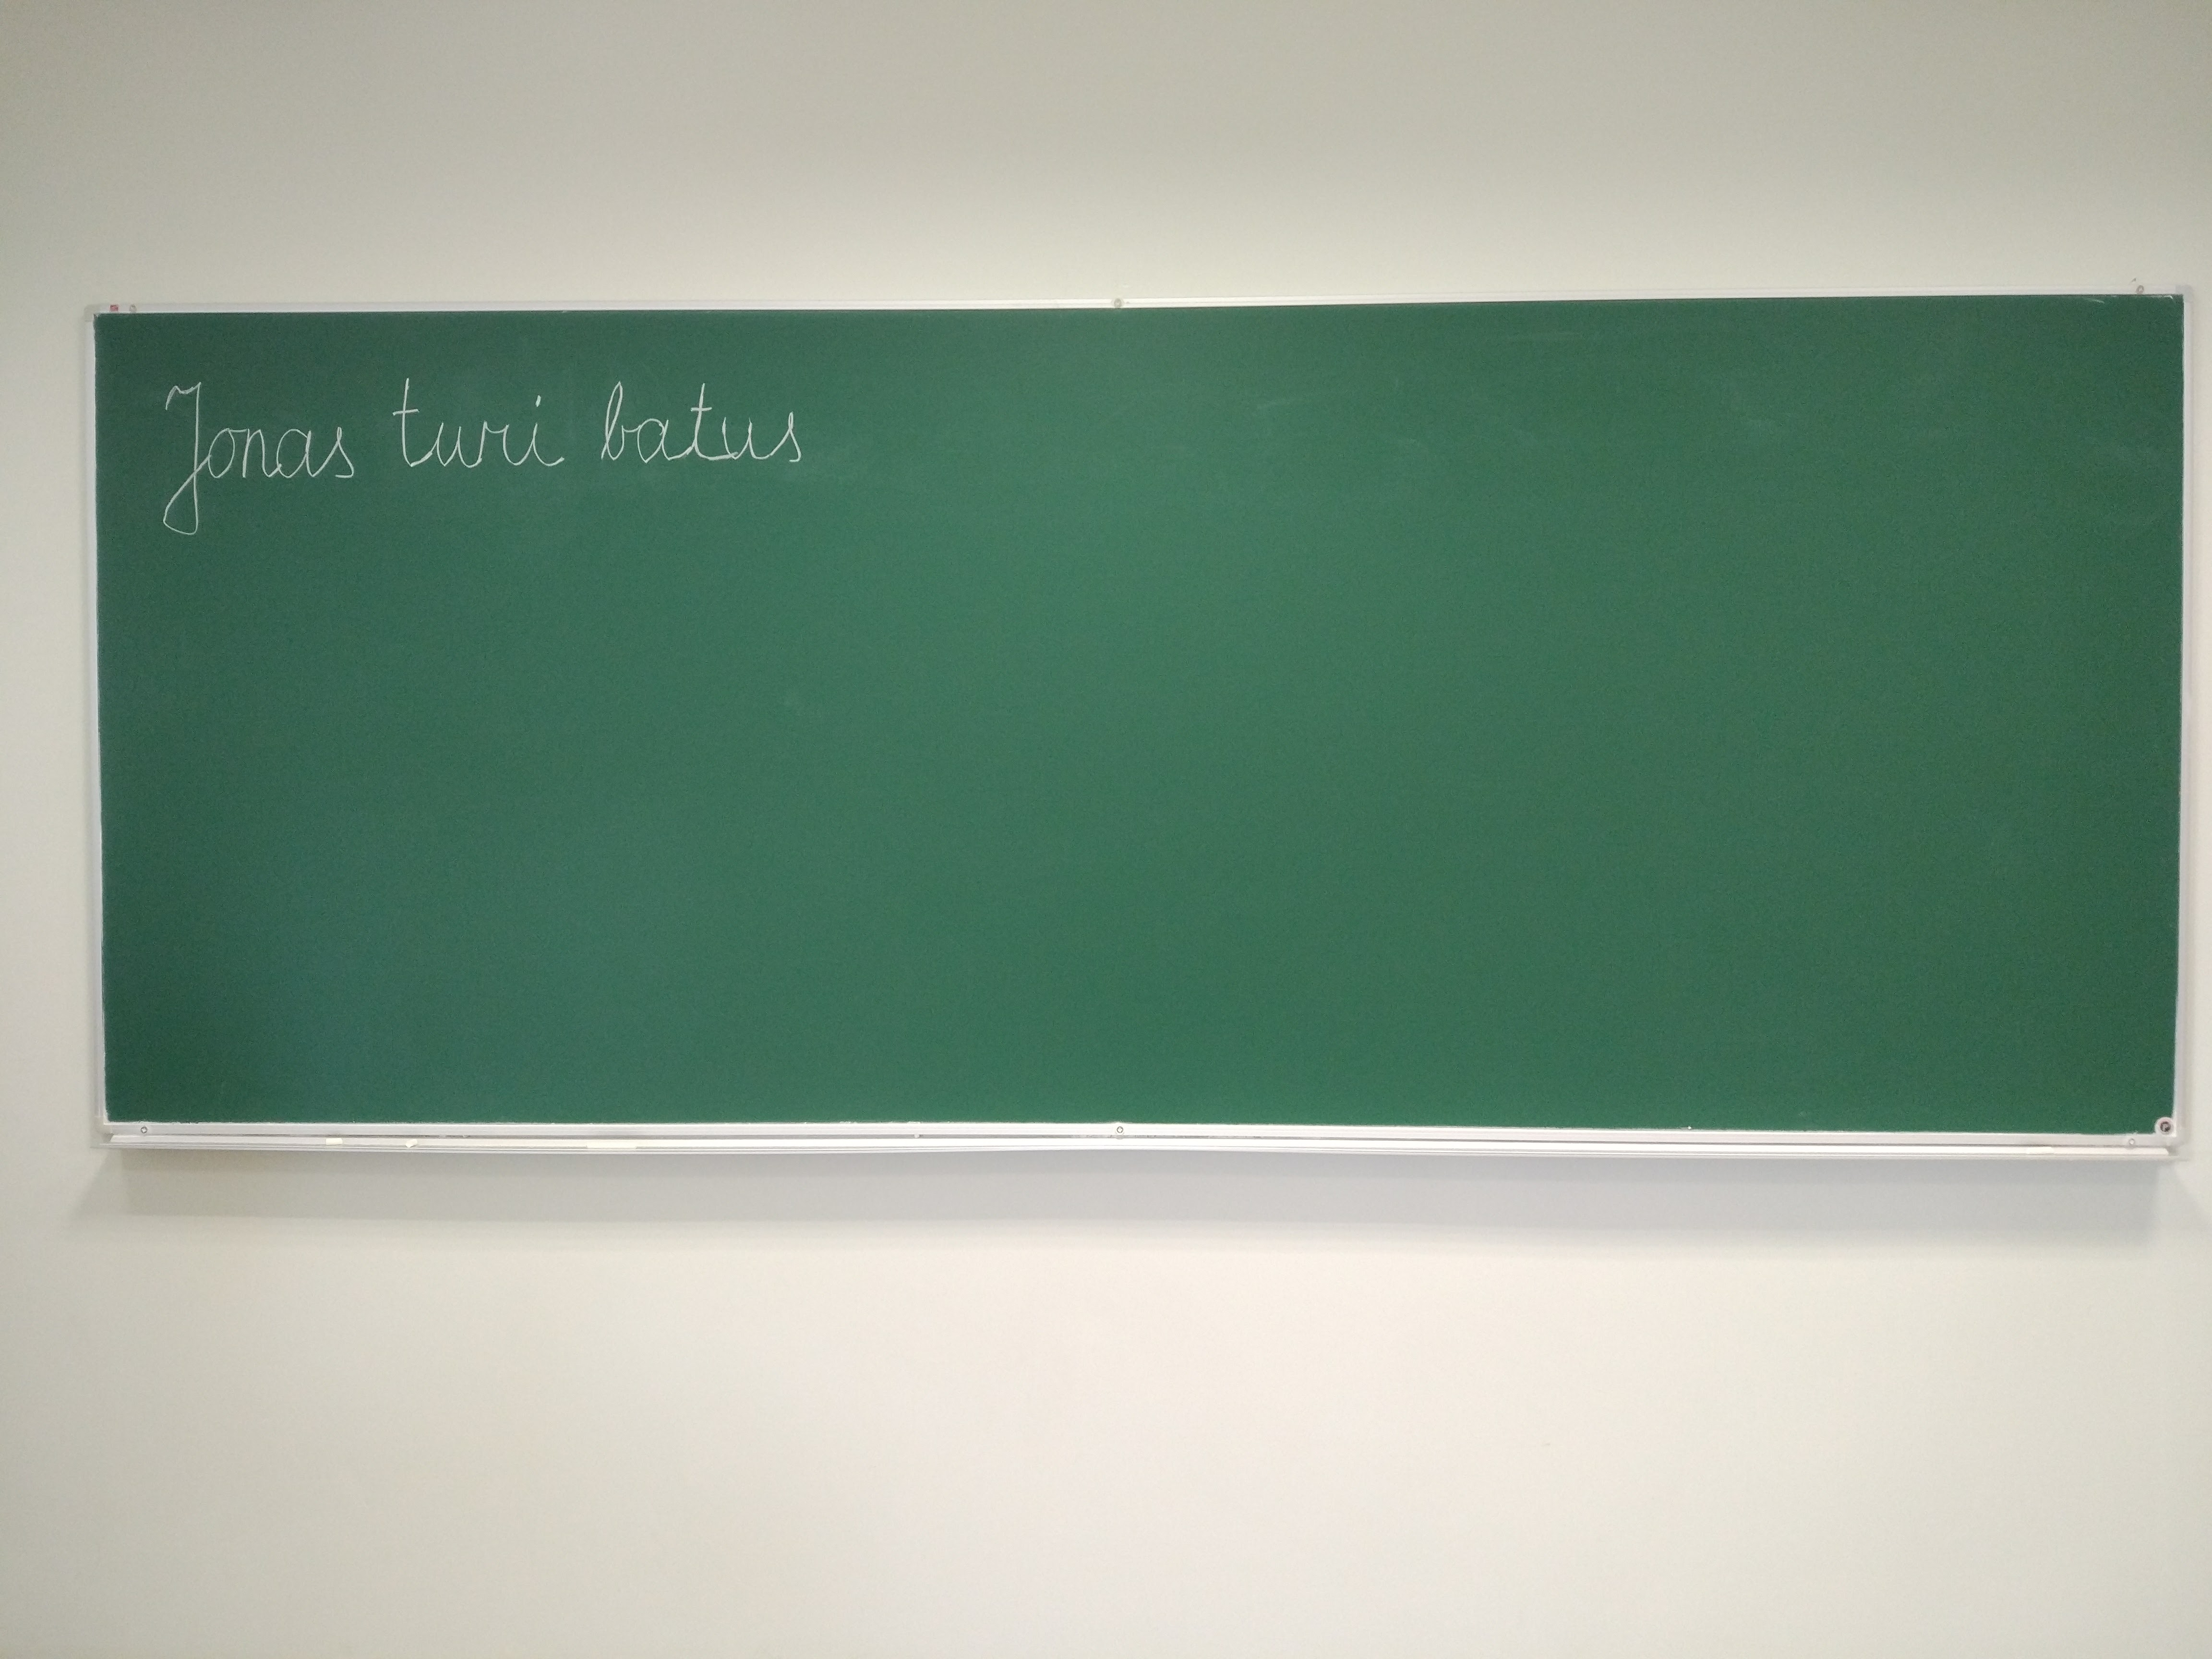
\includegraphics[scale=0.6]{images/test1}
		\caption{Pirmojo bandymo atvaizdo žodžių segmentavimas į atskiras raides.}   % Antraštė įterpiama po paveikslėlio
		\label{img:test1}
	\end{figure}

Tarpiniai rezultatai rodo, kad KNN algoritmas atpažino žodžius „Jonccs“, „tuni“, „hetus“. Pastebima, kad dalis raidžių buvo identifikuotos klaidingai – „a“ kaip „c“ ir „c“, „r“ kaip „n“, „b“ kaip „h“ ir „a“ kaip „e“.

Įvykdžius paiešką žodyne, iš pirmo karto atpažinti žodžiai „Jonas“ ir „turi“. Tačiau „hetus“ atpažintas klaidingai, tad ir galutinis paieškos rezultatas neteisingas – gauti variantai „pietus“, „lietus“ ir „sotus“.

Antrojo bandymo metu analizuojamas atvaizdas \textit{test2.png}. Jame parašyti žodžiai „Ar“, „lis“ ir „rytoj“.
	\begin{figure}[H]
		\centering
		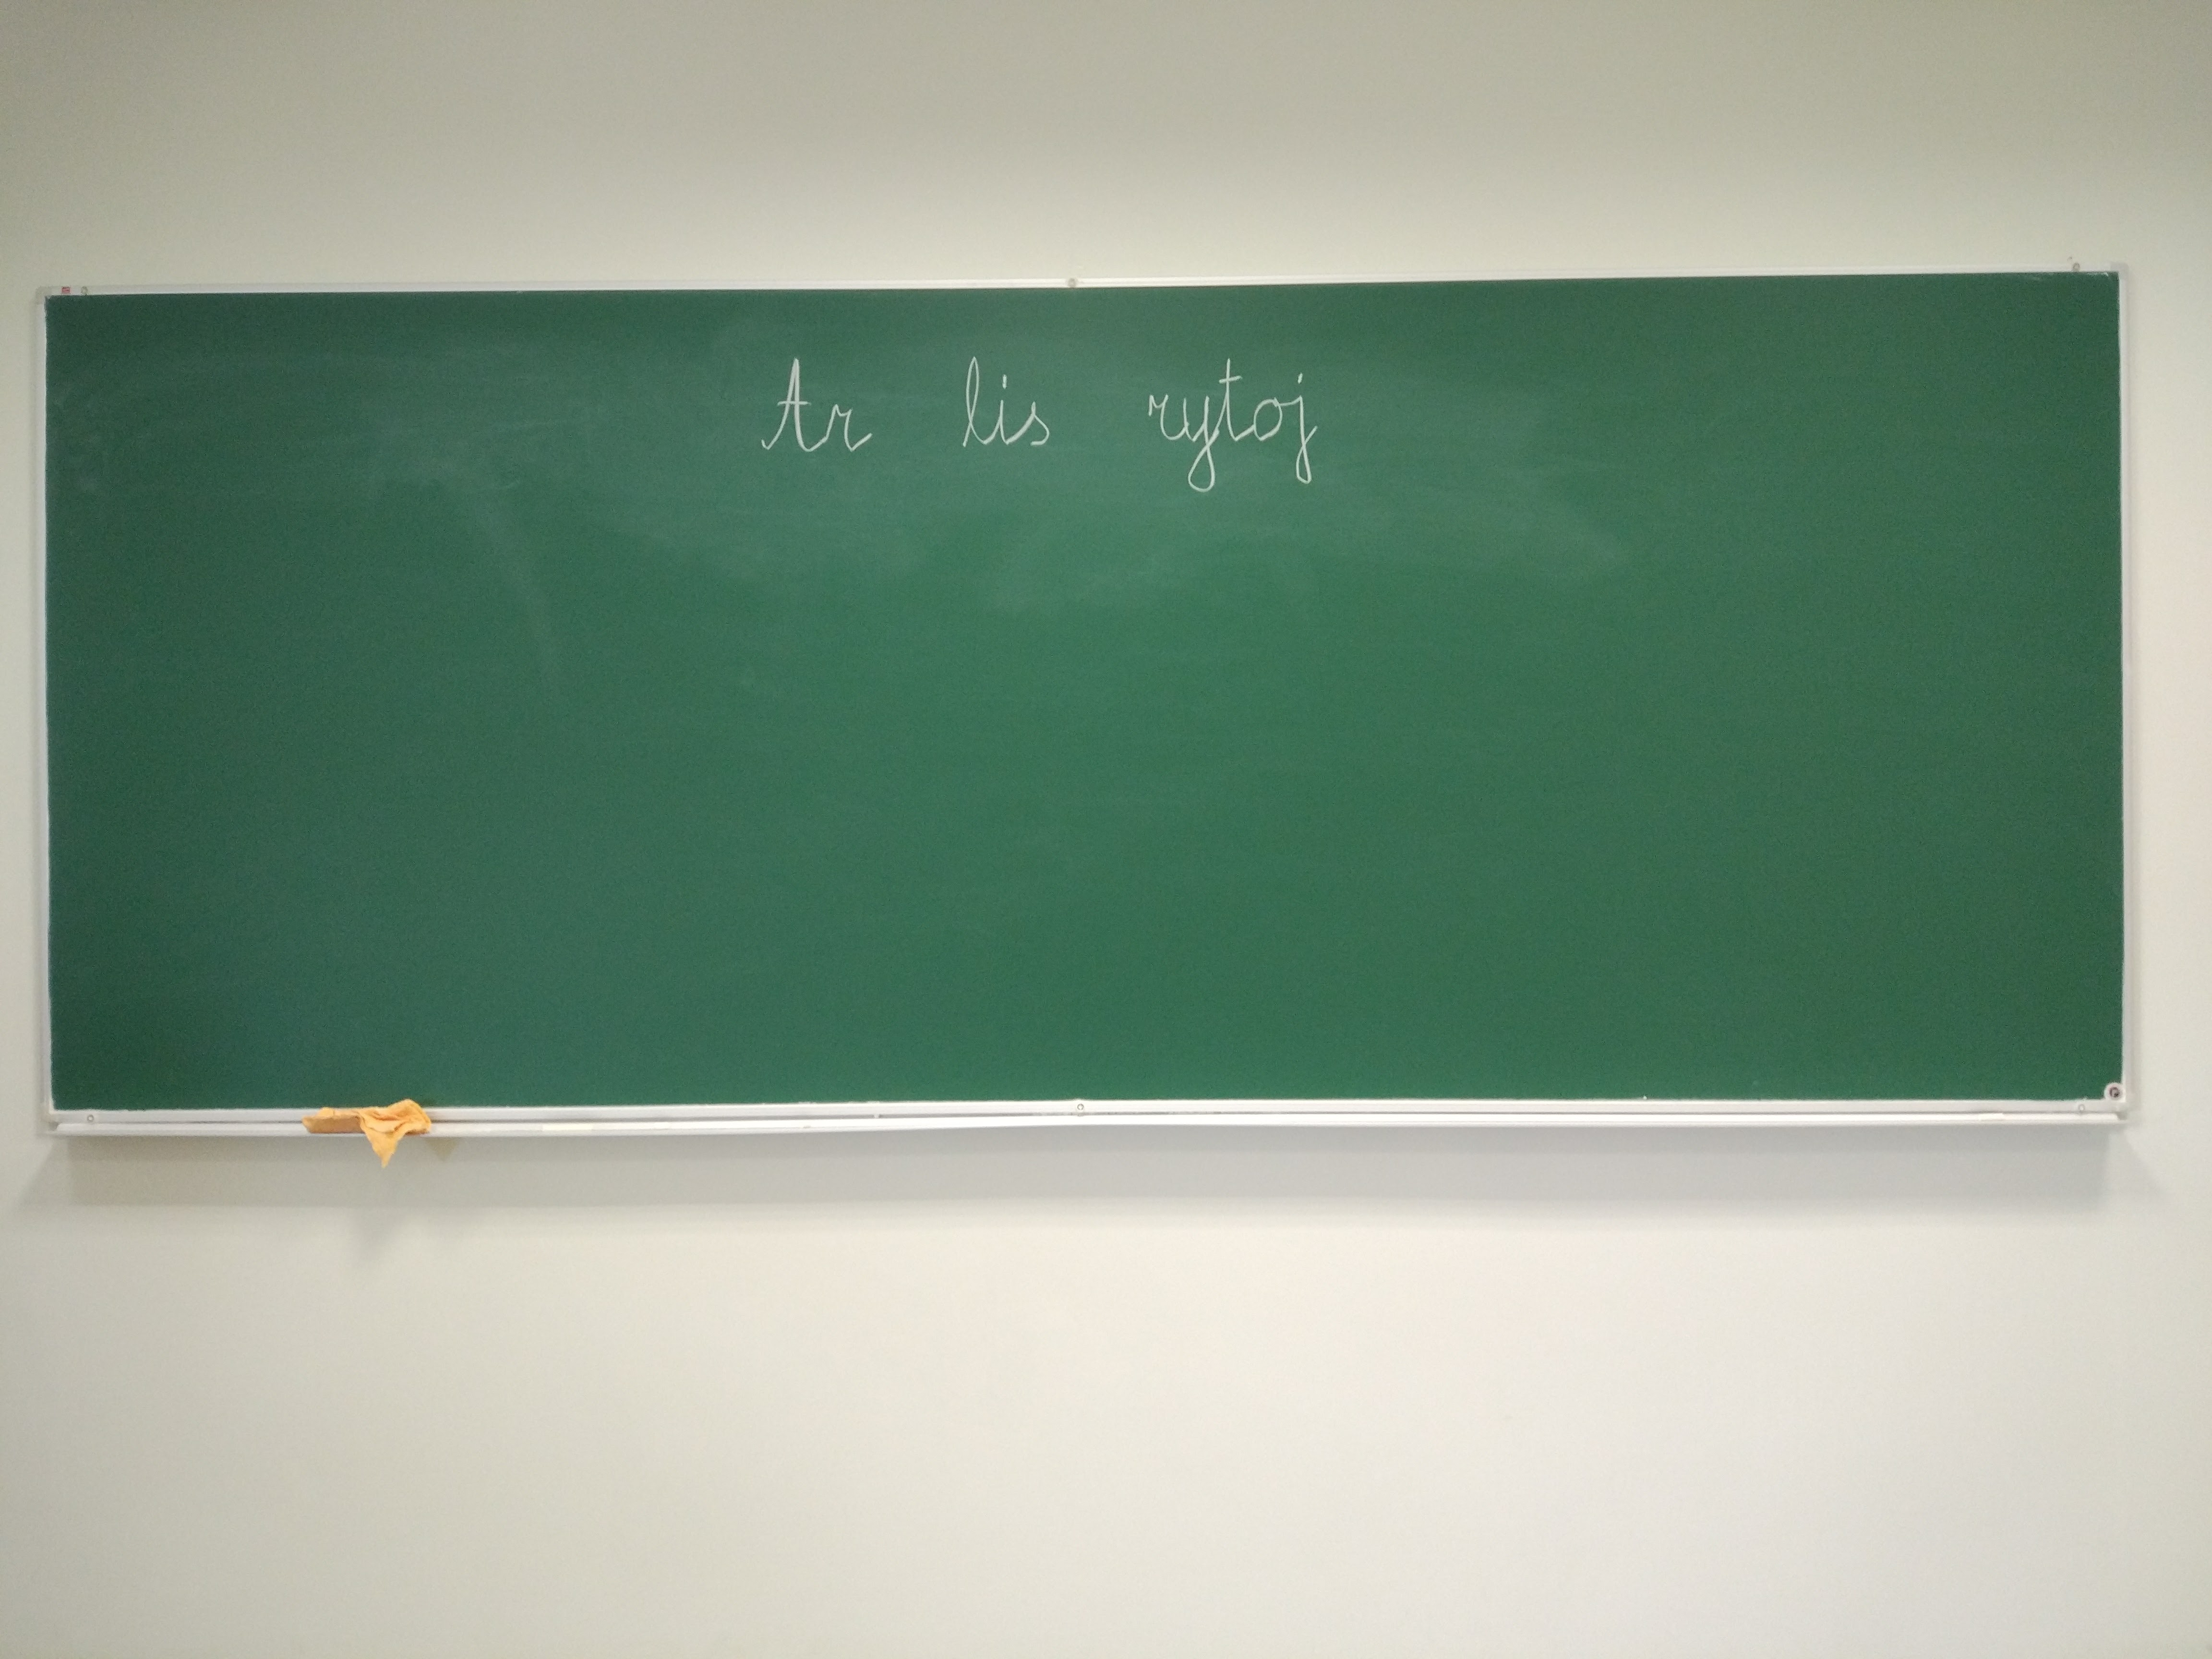
\includegraphics[scale=0.6]{images/test2}
		\caption{Antrojo bandymo atvaizdo žodžių padalijimas į raides.}   % Antraštė įterpiama po paveikslėlio
		\label{img:test2}
	\end{figure}

Gauti tarpiniai rezultatai – „ar“, „lės“ ir „ryboj“. Šiuo atveju „i“ identifikuota kaip „ė“ ir „t“ – kaip „b“. Paieška žodyne grąžina „ar“ bei „rytoj“ kaip pirmąjį galimą variantą. Tuo tarpu „lis“ yra grąžinamas tik kaip trečiasis variantas.

Dalyje bandymų rankraštis atpažįstamas sėkmingai ir beveik be klaidų. Pavyzdžiui, analizuojamas \textit{test9.png} atvaizdas. Jame ant lentos parašyti žodžiai „Brangi“ ir „dovana“.
	\begin{figure}[H]
		\centering
		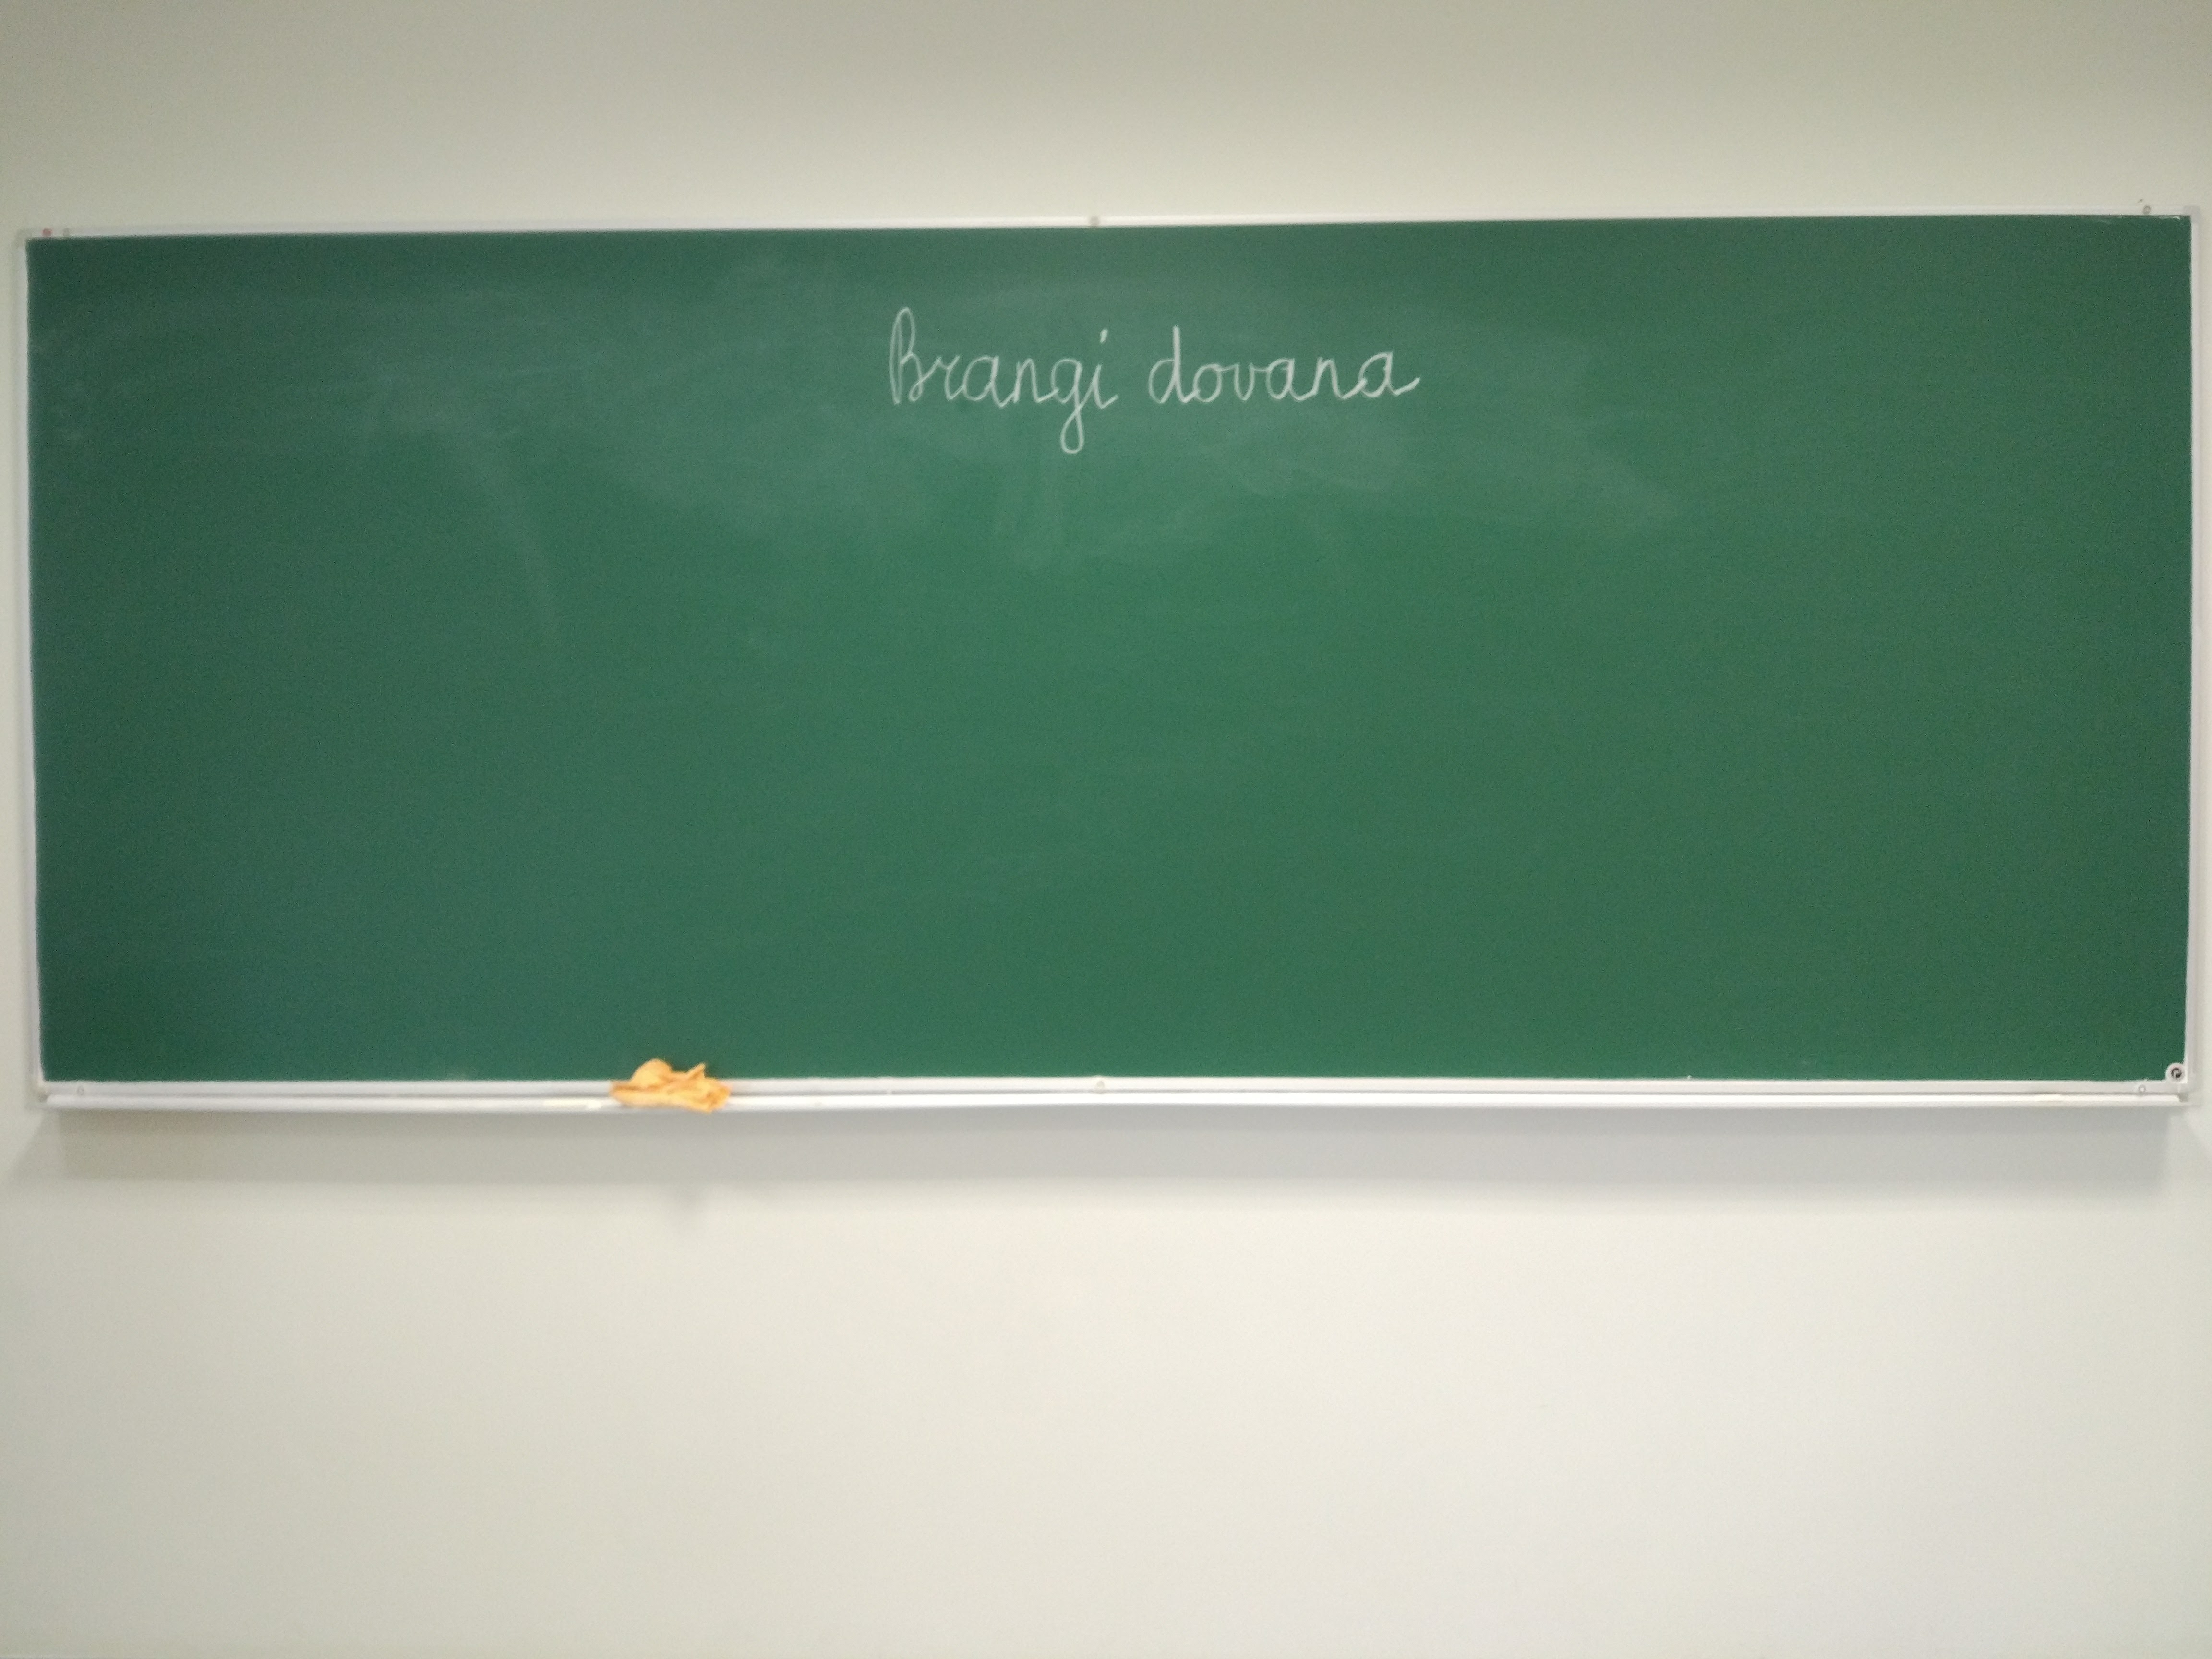
\includegraphics[scale=0.6]{images/test9}
		\caption{Sėkmingo atvaizde esančių žodžių skirstymo į raides pavyzdys.}   % Antraštė įterpiama po paveikslėlio
		\label{img:test9}
	\end{figure}

Įvykdžius programą iš gauto vaizdo matoma, kad suskirstymas į raides atliktas sėkmingai. Tarpiniai rezultatai – „Brungi“ ir „dovana“. Sėkmingai atpažintos visos raidės, išskyrus vieną – vietoje „a“ buvo identifikuota „u“. Tačiau įvykdžius paiešką žodyne ši klaida ištaisoma ir abu žodžiai atpažinti teisingai.

Toliau analogiškai vykdomi bandymai su kitais atvaizdais ir fiksuojami gauti rezultatai.

\subsection{Algoritmo trūkumai}
\paragraph{} Ne visi bandymai buvo tokie sėkmingi. Dalis jų atskleidė algoritmo trūkumus. Analizuojant atvaizdą \textit{test12.png} į iteruojamą kontūrų masyvą įtraukti žodžiai „Lindo“, „kišenę“, tačiau neįtrauktas „į“.
 	\begin{figure}[H]
 		\centering
 		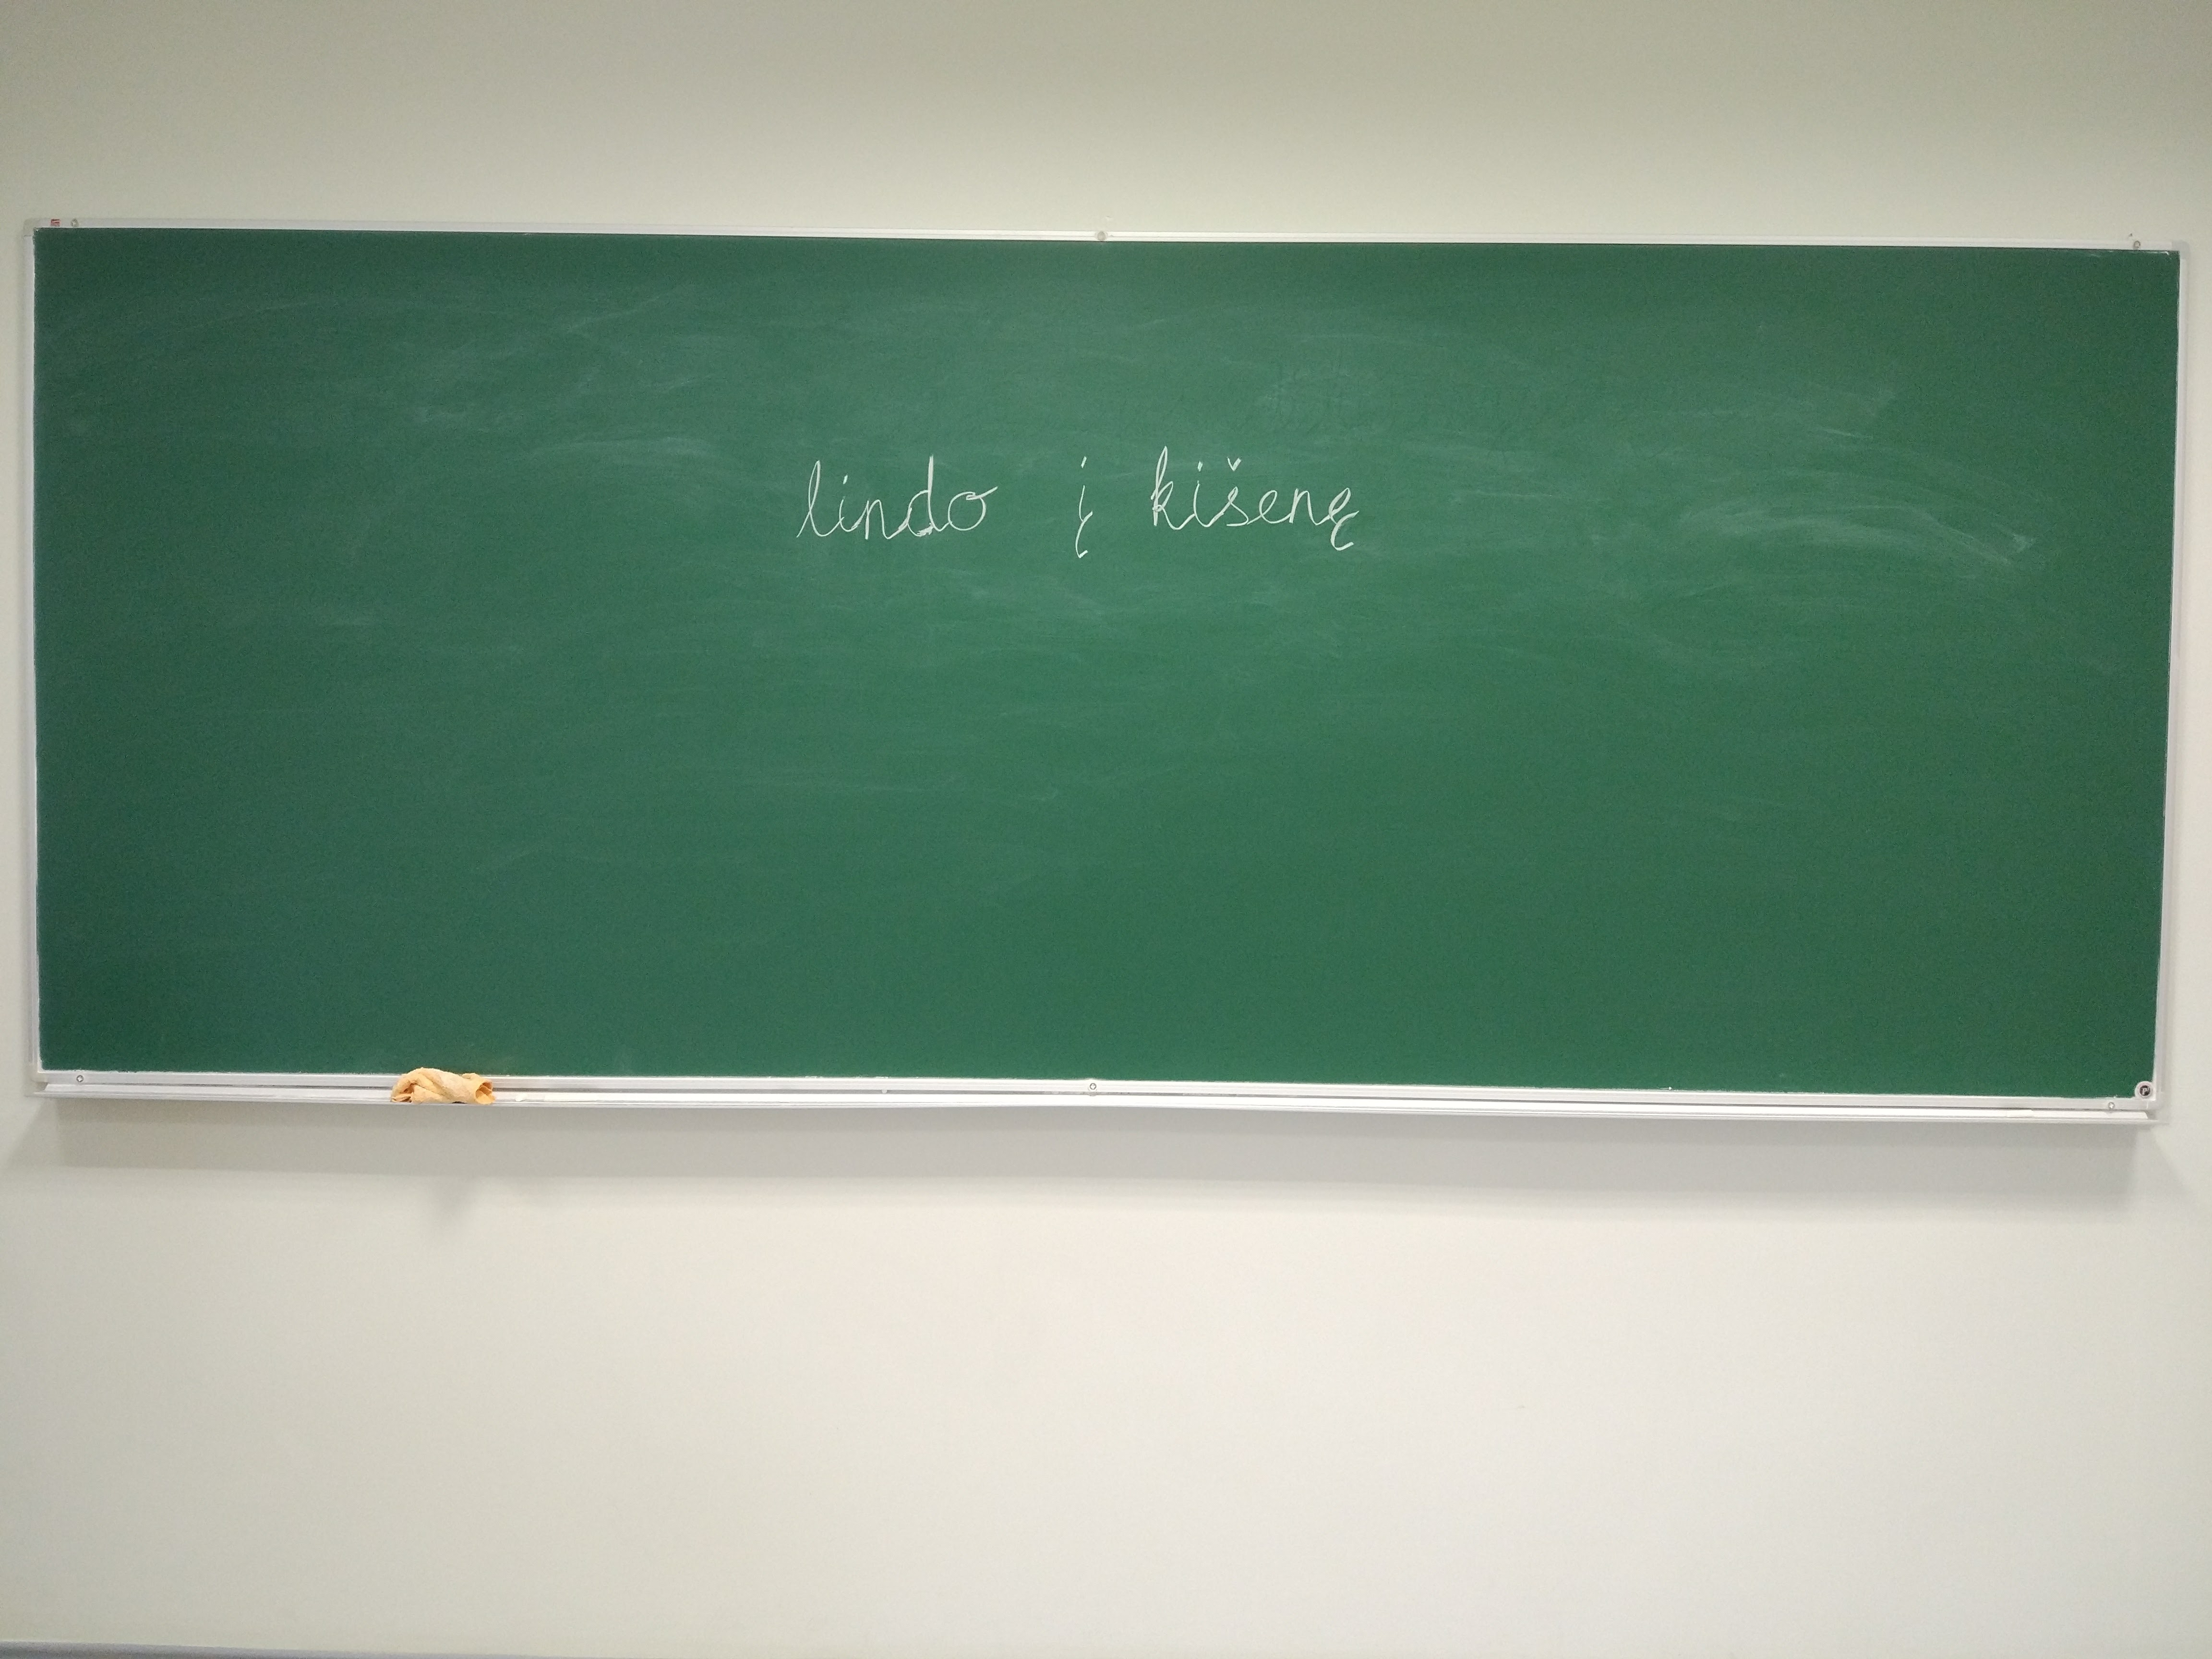
\includegraphics[scale=0.6]{images/test12}
 		\caption{Neteisingai atmestas kontūras, kurio viduje yra žodis.}   % Antraštė įterpiama po paveikslėlio
 		\label{img:test12}
 	\end{figure}

Kontūras neįtrauktas į teksto atpažinimo algoritmą, nes yra per mažo dydžio. Taip atsitinka dėl to, kad nustatyti galimi žodžio dydžio parametrai neatitinka žodžio „į“ aukščio ir pločio.

Atliekant bandymus nustatyta, kad algoritmas neatpažįsta dalies raidžių, nors ir žodis segmentuojamas sėkmingai. Analizuojant \textit{test14.png} paveikslėlį teisingai atpažįstamas tik žodis „bėgti“. KNN algoritmas neteisingai nustato reikšmes žodžiui „puolė“, nors jis ir suskirstytas tinkamai. Dėl šios priežasties paieška žodyne irgi vykdoma pagal neteisingą užklausą. Vietoj teisingo atsakymo gaunami variantai „ne“, „vėl“ ir „per“. Taigi, algoritmas ne visada veikia tinkamai.


 	\begin{figure}[H]
 		\centering
 		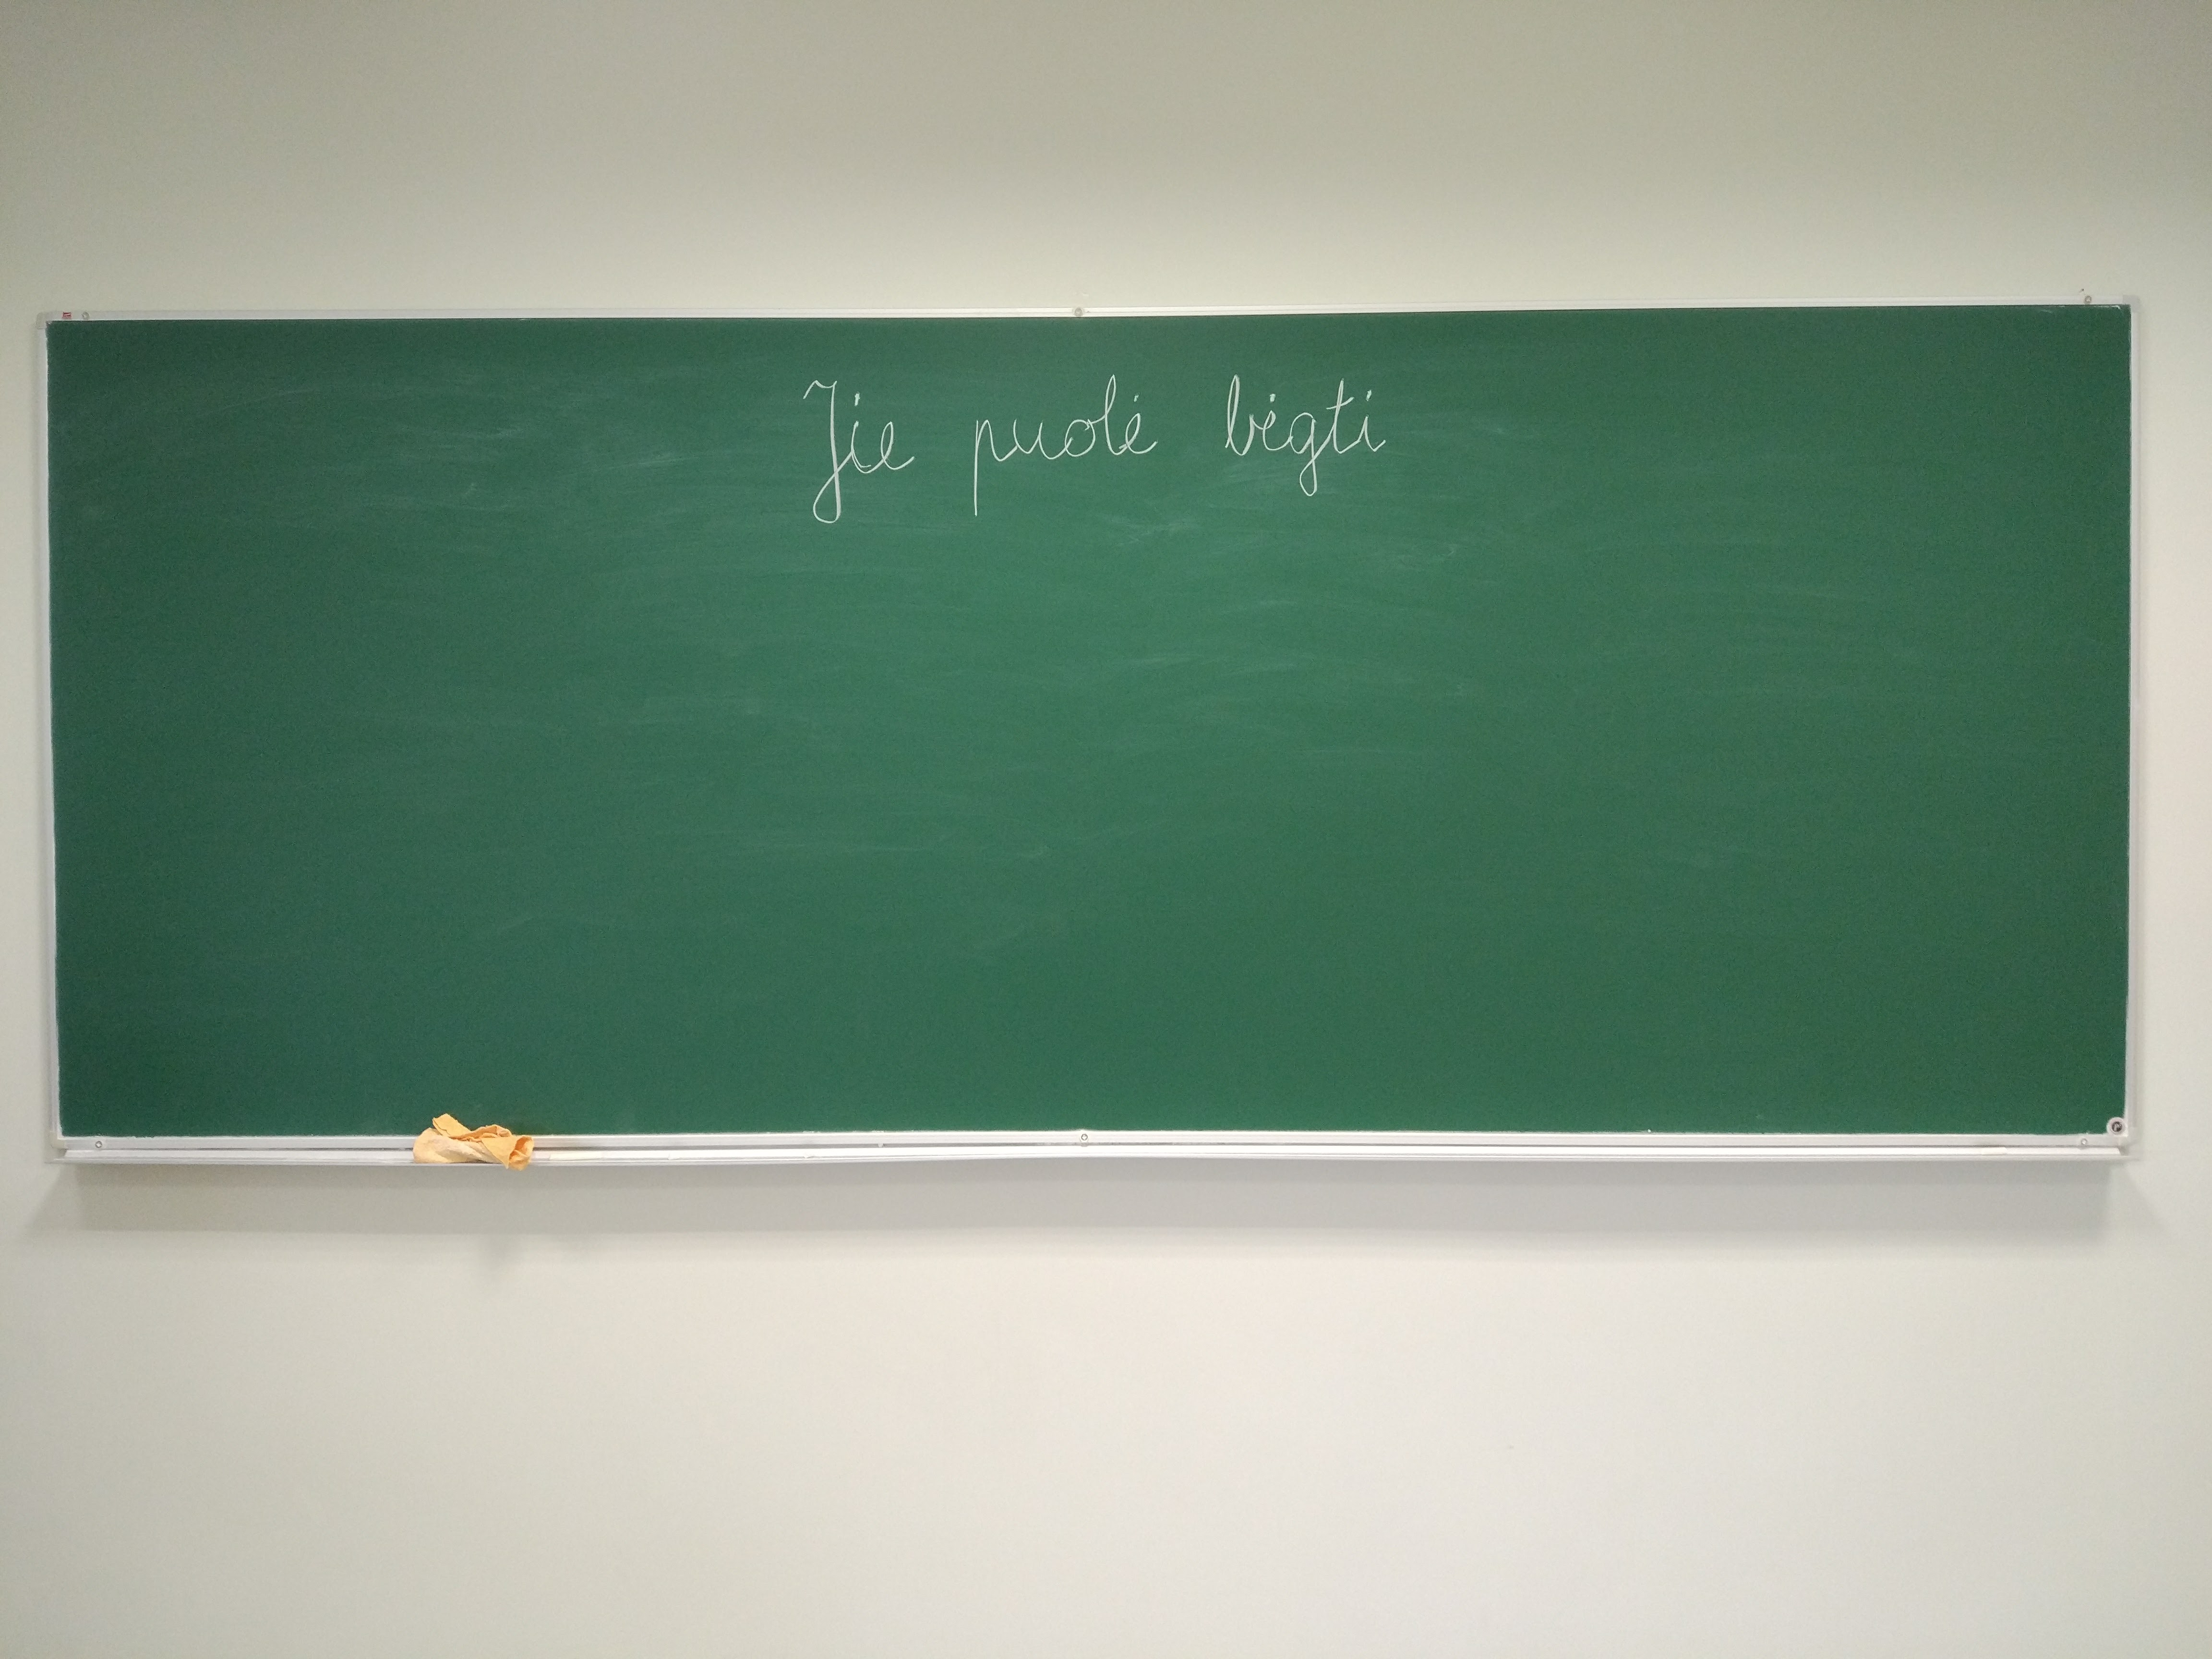
\includegraphics[scale=0.6]{images/test14}
 		\caption{Bandymo metu žodžiai suskirstomi į raides tinkamai, bet atpažinimas nesėkmingas.}   % Antraštė įterpiama po paveikslėlio
 		\label{img:test14}
 	\end{figure}
 	
\subsection{Eksperimento rezultatai}
\paragraph{} Eksperimento metu programos prototipo veikimas buvo išbandytas analizuojant 21 atvaizdą, kuriuose buvo užrašyta 100 atsitiktinai atrinktų žodžių iš sudaryto žodyno. Algoritmas teisingai atpažino 74 žodžius, kai iš žodyno paieškos buvo grąžinamas tik vienas žodis, labiausiai panašus į duotąjį. Septyni žodžiai buvo teisingai atpažinti, kai žodyno paieška grąžino du panašiausių žodžių variantus. Taip pat vienas žodis buvo tinkamai atpažintas, kai paieškos algoritmas grąžino 3 galimus variantus.
Dėl algoritmo trūkumų apskritai nebuvo atpažinta 18 žodžių. Išsamūs rezultatai pateikiami 1-oje lentelėje.

\begin{table}[H]
% Please add the following required packages to your document preamble:
% \usepackage{multirow}
	\centering
	\label{my-label}
	\begin{tabular}{llllll}
		\hline
		\multicolumn{1}{|l|}{\multirow{2}{*}{\textbf{\begin{tabular}[c]{@{}l@{}}Failo\\ vardas\end{tabular}}}} & \multicolumn{3}{l|}{\textbf{Atpažinta kaip:}}                                                                                                                                                                                                                              & \multicolumn{1}{l|}{\multirow{2}{*}{\textbf{\begin{tabular}[c]{@{}l@{}}Neatpažinta\\ žodžių\end{tabular}}}} & \multicolumn{1}{l|}{\multirow{2}{*}{\textbf{\begin{tabular}[c]{@{}l@{}}Bendras\\ žodžių\\ skaičius\end{tabular}}}} \\ \cline{2-4}
		\multicolumn{1}{|l|}{}                                                                                 & \multicolumn{1}{l|}{\textbf{\begin{tabular}[c]{@{}l@{}}1-as\\ variantas\end{tabular}}} & \multicolumn{1}{l|}{\textbf{\begin{tabular}[c]{@{}l@{}}2-as \\ variantas\end{tabular}}} & \multicolumn{1}{l|}{\textbf{\begin{tabular}[c]{@{}l@{}}3-as \\ variantas\end{tabular}}} & \multicolumn{1}{l|}{}                                                                                       & \multicolumn{1}{l|}{}                                                                                              \\ \hline
		\multicolumn{1}{|l|}{test1.png}                                                                        & \multicolumn{1}{l|}{2}                                                                 & \multicolumn{1}{l|}{0}                                                                  & \multicolumn{1}{l|}{0}                                                                  & \multicolumn{1}{l|}{1}                                                                                      & \multicolumn{1}{l|}{3}                                                                                             \\ \hline
		\multicolumn{1}{|l|}{test2.png}                                                                        & \multicolumn{1}{l|}{2}                                                                 & \multicolumn{1}{l|}{0}                                                                  & \multicolumn{1}{l|}{1}                                                                  & \multicolumn{1}{l|}{0}                                                                                      & \multicolumn{1}{l|}{3}                                                                                             \\ \hline
		\multicolumn{1}{|l|}{test3.png}                                                                        & \multicolumn{1}{l|}{3}                                                                 & \multicolumn{1}{l|}{0}                                                                  & \multicolumn{1}{l|}{0}                                                                  & \multicolumn{1}{l|}{0}                                                                                      & \multicolumn{1}{l|}{3}                                                                                             \\ \hline
		\multicolumn{1}{|l|}{test4.png}                                                                        & \multicolumn{1}{l|}{3}                                                                 & \multicolumn{1}{l|}{0}                                                                  & \multicolumn{1}{l|}{0}                                                                  & \multicolumn{1}{l|}{0}                                                                                      & \multicolumn{1}{l|}{3}                                                                                             \\ \hline
		\multicolumn{1}{|l|}{test5.png}                                                                        & \multicolumn{1}{l|}{2}                                                                 & \multicolumn{1}{l|}{1}                                                                  & \multicolumn{1}{l|}{0}                                                                  & \multicolumn{1}{l|}{3}                                                                                      & \multicolumn{1}{l|}{6}                                                                                             \\ \hline
		\multicolumn{1}{|l|}{test6.png}                                                                        & \multicolumn{1}{l|}{8}                                                                 & \multicolumn{1}{l|}{0}                                                                  & \multicolumn{1}{l|}{0}                                                                  & \multicolumn{1}{l|}{1}                                                                                      & \multicolumn{1}{l|}{9}                                                                                             \\ \hline
		\multicolumn{1}{|l|}{test7.png}                                                                        & \multicolumn{1}{l|}{3}                                                                 & \multicolumn{1}{l|}{0}                                                                  & \multicolumn{1}{l|}{0}                                                                  & \multicolumn{1}{l|}{0}                                                                                      & \multicolumn{1}{l|}{3}                                                                                             \\ \hline
		\multicolumn{1}{|l|}{test8.png}                                                                        & \multicolumn{1}{l|}{2}                                                                 & \multicolumn{1}{l|}{0}                                                                  & \multicolumn{1}{l|}{0}                                                                  & \multicolumn{1}{l|}{1}                                                                                      & \multicolumn{1}{l|}{3}                                                                                             \\ \hline
		\multicolumn{1}{|l|}{test9.png}                                                                        & \multicolumn{1}{l|}{2}                                                                 & \multicolumn{1}{l|}{0}                                                                  & \multicolumn{1}{l|}{0}                                                                  & \multicolumn{1}{l|}{0}                                                                                      & \multicolumn{1}{l|}{2}                                                                                             \\ \hline
		\multicolumn{1}{|l|}{test10.png}                                                                       & \multicolumn{1}{l|}{7}                                                                 & \multicolumn{1}{l|}{0}                                                                  & \multicolumn{1}{l|}{0}                                                                  & \multicolumn{1}{l|}{1}                                                                                      & \multicolumn{1}{l|}{8}                                                                                             \\ \hline
		\multicolumn{1}{|l|}{test11.png}                                                                       & \multicolumn{1}{l|}{2}                                                                 & \multicolumn{1}{l|}{0}                                                                  & \multicolumn{1}{l|}{0}                                                                  & \multicolumn{1}{l|}{0}                                                                                      & \multicolumn{1}{l|}{2}                                                                                             \\ \hline
		\multicolumn{1}{|l|}{test12.png}                                                                       & \multicolumn{1}{l|}{2}                                                                 & \multicolumn{1}{l|}{0}                                                                  & \multicolumn{1}{l|}{0}                                                                  & \multicolumn{1}{l|}{1}                                                                                      & \multicolumn{1}{l|}{3}                                                                                             \\ \hline
		\multicolumn{1}{|l|}{test13.png}                                                                       & \multicolumn{1}{l|}{7}                                                                 & \multicolumn{1}{l|}{1}                                                                  & \multicolumn{1}{l|}{0}                                                                  & \multicolumn{1}{l|}{1}                                                                                      & \multicolumn{1}{l|}{9}                                                                                             \\ \hline
		\multicolumn{1}{|l|}{test14.png}                                                                       & \multicolumn{1}{l|}{1}                                                                 & \multicolumn{1}{l|}{0}                                                                  & \multicolumn{1}{l|}{0}                                                                  & \multicolumn{1}{l|}{2}                                                                                      & \multicolumn{1}{l|}{3}                                                                                             \\ \hline
		\multicolumn{1}{|l|}{test15.png}                                                                       & \multicolumn{1}{l|}{6}                                                                 & \multicolumn{1}{l|}{2}                                                                  & \multicolumn{1}{l|}{0}                                                                  & \multicolumn{1}{l|}{1}                                                                                      & \multicolumn{1}{l|}{9}                                                                                             \\ \hline
		\multicolumn{1}{|l|}{test16.png}                                                                       & \multicolumn{1}{l|}{3}                                                                 & \multicolumn{1}{l|}{0}                                                                  & \multicolumn{1}{l|}{0}                                                                  & \multicolumn{1}{l|}{0}                                                                                      & \multicolumn{1}{l|}{3}                                                                                             \\ \hline
		\multicolumn{1}{|l|}{test17.png}                                                                       & \multicolumn{1}{l|}{1}                                                                 & \multicolumn{1}{l|}{1}                                                                  & \multicolumn{1}{l|}{0}                                                                  & \multicolumn{1}{l|}{1}                                                                                      & \multicolumn{1}{l|}{3}                                                                                             \\ \hline
		\multicolumn{1}{|l|}{test18.png}                                                                       & \multicolumn{1}{l|}{5}                                                                 & \multicolumn{1}{l|}{0}                                                                  & \multicolumn{1}{l|}{0}                                                                  & \multicolumn{1}{l|}{1}                                                                                      & \multicolumn{1}{l|}{6}                                                                                             \\ \hline
		\multicolumn{1}{|l|}{test19.png}                                                                       & \multicolumn{1}{l|}{2}                                                                 & \multicolumn{1}{l|}{0}                                                                  & \multicolumn{1}{l|}{0}                                                                  & \multicolumn{1}{l|}{1}                                                                                      & \multicolumn{1}{l|}{3}                                                                                             \\ \hline
		\multicolumn{1}{|l|}{test20.png}                                                                       & \multicolumn{1}{l|}{6}                                                                 & \multicolumn{1}{l|}{1}                                                                  & \multicolumn{1}{l|}{0}                                                                  & \multicolumn{1}{l|}{2}                                                                                      & \multicolumn{1}{l|}{9}                                                                                             \\ \hline
		\multicolumn{1}{|l|}{test21.png}                                                                       & \multicolumn{1}{l|}{5}                                                                 & \multicolumn{1}{l|}{1}                                                                  & \multicolumn{1}{l|}{0}                                                                  & \multicolumn{1}{l|}{1}                                                                                      & \multicolumn{1}{l|}{7}                                                                                             \\ \hline
		& \textbf{}                                                                              & \textbf{}                                                                               & \textbf{}                                                                               & \textbf{}                                                                                                   & \textbf{}                                                                                                          \\ \hline
		\multicolumn{1}{|l|}{\textbf{Viso:}}                                                                   & \multicolumn{1}{l|}{\textbf{74}}                                                       & \multicolumn{1}{l|}{\textbf{7}}                                                         & \multicolumn{1}{l|}{\textbf{1}}                                                         & \multicolumn{1}{l|}{\textbf{18}}                                                                            & \multicolumn{1}{l|}{\textbf{100}}                                                                                  \\ \hline
	\end{tabular}
	\caption{Eksperimento rezultatai.}
\end{table}

Buvo apskaičiuotas vidurkis, kokiu tikslumu vidutiniškai atpažįstami lietuvių kalbos žodžiai iš šio darbo autoriaus pasirinkto 250 žodžių žodyno. Tam naudota ši euristinė formulė: 

\[ E(X_n) = \frac{x_1 + \frac{1}{2}x_2 + \frac{1}{3}x_3}{100} \]

$x_1$ – teisingai atpažintų žodžių skaičius, kai grąžinamas tik vienas variantas.

$x_2$ – teisingai atpažintų žodžių skaičius, kai grąžinami du galimi variantai.

$x_2$ – teisingai atpažintų žodžių skaičius, kai grąžinami trys galimi variantai.

Formulėje prie $x_2$ ir $x_3$ kintamųjų nurodyti koeficientai \(\frac{1}{2}\) ir \(\frac{1}{3}\). Jie suteikia skirtingas vertes algoritmo grąžinamiems atitinkamai dviems ir trims panašiausiems žodžiams. Taip yra todėl, jog laikoma, kad algoritmui grąžinant du žodžių variantus ir atsitiktinai renkantis vieną teisingą – teisingo žodžio gavimo tikimybė yra lygi \(\frac{1}{2}\). Analogiškai, tikimybė yra lygi \(\frac{1}{3}\), kai grąžinami trys variantai.
 
Naudojant bandymų rezultatus apskačiuota, kad tikimybinis vidurkis, jog žodis bus atpažintas teisingai yra \( 0.7783 \).


\clearpage
\section*{Išvados}
\addcontentsline{toc}{section}{Išvados}
\paragraph{}Šiame darbe buvo apžvelgti kompiuterinės regos praktiniai taikymai. Pristatyta populiari ir plačiai naudojama bei daug funkcijų turinti kompiuterinės regos biblioteka OpenCV. Taip pat trumpai apžvelgtos jos funkcijos, naudojamos vaizdų apdorojimui ir mašininiam mokymui. Buvo suformuluotas darbo tikslas – atpažinti lietuvių kalbos rankraštį. Minėtas tikslas praktinėje dalyje buvo sprendžiamas sukuriant lietuvių kalbos žodžių atpažinimo algoritmą, parašytą Python programavimo kalba. Algoritmo įgyvendinimui naudotos OpenCV bibliotekos vaizdų apdorojimo, mašininio mokymo funkcijos. Taip pat – Python programavimo kalbos numpy, os, sys, difflib, time paketai. Buvo sukurtas ir mašininiam mokymui panaudotas mokymosi duomenų rinkinys, sudarytas iš lietuvių kalbos raidžių atvaizdų.
 
Algoritmo veikimas buvo išbandytas atliekant praktinį eksperimentą. Atvaizdai, naudoti eksperimente gauti keliose Vilniaus Universiteto Matematikos ir Informatikos fakulteto auditorijose. Tuose atvaizduose užfiksuoti auditorijos lentoje užrašyti lietuviško teksto fragmentai. Pritaikius KNN mašininio mokymo algoritmą ir tikslinamąją paiešką riboto dydžio žodyne programos prototipas teisingai atpažino žodžius tikimybiniu vidurkiu \( 0.7783 \).

Atliekant praktinį eksperimentą išryškėjo ir programos prototipo trūkumai. Šiuo metu algoritmas tinkamai veikia tik su darbo autoriaus parašytu lietuvišku rankraščiu. Taip pat analizuojami atvaizdai turi būti užfiksuoti esant pastoviam dirbtiniam apšvietimui. Žodžių suskirstymas į raides ir pačių raidžių identifikavimas ne visada vyko tiksliai dėl sąlyginai nedidelio mokymosi duomenų rinkinio dydžio ir pasirinkto sąlyginai nesudėtingo mašininio mokymo KNN algoritmo.

Sukurto programos prototipo praktinio panaudojimo potencialas yra didelis, todėl ateityje jį galima tobulinti. Geresniam algoritmo veikimui reikalingas bent keliolika kartų didesnis mokymosi duomenų rinkinys. Taip pat galima pakeisti KNN mašininio mokymo algoritmą į efektyvesnį, pavyzdžiui, neuroninį tinklą. Kitas rankraščio atpažinimo tikslumo pagerinimo būdas gali būti papildomas mašininio mokymo naudojimas žodžių atpažinimui arba raidžių susijungimo vietoms aptikti taip patikslinant žodžių skirstymą į raides. Algoritmo panaudojimo galimybes išplėstų ir lankstesnis vaizdo apdorojimas. Tokiu būdu būtų panaikintas reikalavimas fiksuoti atvaizdus specifinėmis sąlygomis. Taip pat programai reikalinga grafinė vartotojo sąsaja norint priimtiniau atvaizduoti rankraščio atpažinimo rezultatus. Prototipas gali būti panaudotas ir kaip pagrindas tokiu pat principu veikiančiai išmaniųjų telefonų programai sukurti.

Šis baigiamasis bakalauro darbas parodo naudingą kompiuterinės regos taikymo galimybę ugdymo įstaigose ar kitose srityse, kur būtina vėlesniam laikui išsaugoti ranka užrašytą informaciją. Tokiu būdu galima išvengti būtinybės užrašus rašyti ranka ir taip pat sutaupyti laiko – palengvinti mokymosi bei darbo procesus.
 
 
\clearpage 
\begin{thebibliography}{99}
\addcontentsline{toc}{section}{Literatūra} %% Literatura bus itraukta i turini
\bibitem {OPENCV}
G. Bradski ir A. Kaehler, \textit{Learning OpenCV: Computer vision with the OpenCV library}, O'Reilly Media, Inc., 2008, p. 1–8.

\bibitem {MALARIA}
N. Linder ir kt., \textit{A malaria diagnostic tool based on computer vision screening and visualization of Plasmodium falciparum candidate areas in digitized blood smears}, PLoS One 9.8 (2014): e104855.

\bibitem {CARPLATE}
E. Christos-Nikolaos Anagnostopoulos ir kt., \textit{License plate recognition from still images and video sequences: A survey}, IEEE Transactions on intelligent transportation systems 9.3 (2008), p. 377-391.

\bibitem {PRADEEP}
J. Pradeep, E. Srinivasan ir S. Himavathi, \textit{Diagonal based feature extraction for handwritten character recognition system using neural network}, Electronics Computer Technology (ICECT), 2011 3rd International Conference IEEE, 2011.

\bibitem{CHINAPOST}
S. Lu ir kt., \textit{Cost-sensitive neural network classifiers for postcode recognition}, International Journal of Pattern Recognition and Artificial Intelligence 26.05 (2012): 1263001.

\bibitem{PEOPLECOUNT}
C. Chen ir kt., \textit{A cost-effective people-counter for a crowd of moving people based on two-stage segmentation}, Journal of Information Hiding and Multimedia Signal Processing 3.1 (2012): 12-25.
 
\bibitem {LeCun}
Y. LeCun ir kt., \textit{Comparison of learning algorithms for handwritten digit recognition}, International conference on artificial neural networks. Vol. 60. 1995, \url{http://yann.lecun.com/exdb/publis/pdf/lecun-95b.pdf}.

\bibitem{PLATEIMG}
D. Kostadinov, \textit{Privacy Implications of Automatic License Plate Recognition Technology}, \url{http://resources.infosecinstitute.com/privacy-implications-automatic-license-plate-recognition-technology/}.

\bibitem{POSTCODE}
 Shujing Lu ir kt., \textit{Cost-sensitive neural network classifiers for postcode recognition}, International Journal of Pattern Recognition and Artificial Intelligence, 2012.
 
\bibitem{CVWEB}
OpenCV kompiuterinės regos bibliotekos žiniatinklio puslapis, \url{http://opencv.org/about.html}.

\bibitem{MORPHOLOGIC}
OpenCV bibliotekos morfologinės transformacijos, \url{http://docs.opencv.org/trunk/d9/d61/tutorial_py_morphological_ops.html}.

\bibitem{CONTOURS}
OpenCV bibliotekos kontūrų radimo funkcijų aprašymas, \url{http://docs.opencv.org/3.1.0/dd/d49/tutorial_py_contour_features.html}.

\bibitem{CVCOLORS}
OpenCV spalvų erdvės transformacijos, \url{http://docs.opencv.org/3.2.0/df/d9d/tutorial_py_colorspaces.html}.

\bibitem{COLORSPACE}
A. Ford ir A. Roberts, \textit{Colour Space Conversions}, 1998,
\url{http://sites.biology.duke.edu/johnsenlab/pdfs/tech/colorconversion.pdf}.

\bibitem{THRESHOLD}
Atvaizdo slenkstinės vertės nustatymas, \url{http://docs.opencv.org/trunk/d7/d4d/tutorial_py_thresholding.html}.

\bibitem{KNN}
KNN algoritmo paaiškinimas, \url{http://opencv-python-tutroals.readthedocs.io/en/latest/py_tutorials/py_ml/py_knn/py_knn_understanding/py_knn_understanding.html#knn-understanding}.

\bibitem{MNIST}
MNIST ranka rašytų skaičių duomenų rinkinys, \url{http://yann.lecun.com/exdb/mnist/}.

\bibitem{MNISTNUMBERS}
MNIST duomenų iliustracija, \url{http://neuralnetworksanddeeplearning.com/images/mnist_2_and_1.png}.

\bibitem{DLKZ}
Dabartinės lietuvių kalbos žodynas, \url{http://lkiis.lki.lt/dabartinis}.

\bibitem{NUMPY}
Python numpy paketo vartotojo gidas, \url{https://docs.scipy.org/doc/numpy-dev/user/quickstart.html}.

\bibitem{SYS}
Python sys paketo dokumentacija, \url{https://docs.python.org/3/library/sys.html}.

\bibitem{OS}
Python os paketo dokumentacija, \url{https://docs.python.org/3/library/os.html}.

\bibitem{DIFFLIB}
Python difflib paketo dokumentacija, \url{https://docs.python.org/2/library/difflib.html}.

\end{thebibliography} 
 
\clearpage 
\section*{Santrauka}
\addcontentsline{toc}{section}{Santrauka}
\paragraph{}Bakalauro darbe „Lietuviško rankraščio atpažinimas ir taikymas“ apžvelgta ir pristatyta kompiuterinės regos ir mašininio mokymo biblioteka OpenCV bei jos funkcijos. Darbe buvo siekiama sukurti programos prototipą, kuris atpažįsta lietuvių kalbos žodžius, parašytus ranka. Prototipas pritaikytas atpažinti universiteto auditorijoje lentoje parašytą tekstą ir vartotojui pateikti rezultatą kompiuterio ekrane.

Darbo tikslas buvo pasiektas. Iš pradžių sukurtas mokymosi duomenų rinkinys iš lietuviškų raidžių atvaizdų. Ruošiant vaizdą analizei, prototipo algoritmas naudoja įvairias vaizdo apdorojimo funkcijas. KNN mašininio mokymo algoritmas naudojamas raidžių identifikavimui, o Python difflib paketo funkcijos naudojamos norint patikslinti, koks žodis atitinka atpažintą raidžių seką.

Buvo atliktas praktinis eksperimentas, kurio metu išanalizuotas prototipo veikimo tikslumas. Taip pat buvo išsiaiškinti prototipo trūkumai bei galimi patobulinimai.
\newline
\newline
\paragraph{}Raktiniai žodžiai: kompiuterinė rega, mašininis mokymas, lietuviško rankraščio atpažinimas, vaizdo apdorojimas, Python, OpenCV, difflib, KNN, mokymosi duomenų rinkinys.


\clearpage
\section*{Summary}
\addcontentsline{toc}{section}{Summary}
\paragraph{}A computer vision and machine learning library OpenCV is presented and reviewed in the bachelor thesis „Lithuanian handwriting recognition and its application“. The main goal of the thesis is to create a prototype of a program, which is capable to recognize a lithuanian handwriting. The prototype is adapted to recognize a text written on a green board in a classroom of the university and it shows the result on the screen of the computer.

The goal was reached. In the beginning, the learning data set was created. It consists of images of the lithuanian alphabet letters. The prototype uses various image processing functions to prepare the image for the analysis. A KNN machine learning algorithm is used to identify letters and a Python difflib package helps to match a word with the recognized sequence of letters. 

There was a practical experiment done in order to analyse the accuracy of the prototype. Also, the weaknesses of the prototype were discovered and the possible improvements for the prototype were presented.
\newline
\newline
\paragraph{}Keywords: computer vision, machine learning, lithuanian handwriting recognition, image processing, Python, OpenCV, difflib, KNN, learning data set.


\clearpage
\pagestyle{empty}
\appendix
\cftaddtitleline{toc}{section}{Priedas}{}
\section*{Priedas}
\subsection*{Programinės įrangos naudojimo instrukcijos}
\paragraph{} Šio darbo elektroninė versija, programos prototipo failai ir eksperimente bei mokymo duomenų ruošime naudoti atvaizdai pateikiami elektroninėje laikmenoje kartu su šiuo darbu. Visi programiniai failai bei jų versijos pasiekiamos ir žiniatinklyje, adresu: \newline
\url{https://github.com/vytjan/final-ml}.

Programos prototipo veikimas išbandytas naudojant kartu pateiktus atvaizdus ir šias programinės įrangos komponentų versijas:
\begin{itemize}
	\item Operacinė sistema – Linux Ubuntu 16.04 versija.
	\item Python 3.5.2 versija.
	\item Python NumPy paketo 1.11.0 versija.
\end{itemize}

Darbo failus sudaro „src“ ir „doc“ aplankai. Aplanke „doc“ yra šio rašto darbo \textit{pdf} ir \textit{tex} formato failai, o „images“ aplanke – darbe naudojamos iliustracijos. \textit{tex} formato failas kompiliuojamas į \textit{pdf} dokumentą vykdant komandą:\newline
\textit{pdflatex -synctex=1 -interaction=nonstopmode} \newline
\textit{--shell-escape "Bakalauro\_darbas\_Vytautas\_Jankauskas".tex}

„src“ aplanke patalpinti darbo praktinėje dalyje naudoti failai. „letters-50“ aplanke patalpintas mokymosi duomenų rinkinys, sukurtas naudojant \textit{classification.py} programą. Programa \textit{learningset.py} sugeneravo \textit{generalsamplesNEW.data} ir \textit{generalresponsesNEW.data} failus. Pagal juos apmokomas KNN algoritmas. \textit{dictionary.data} faile yra darbo autoriaus sudarytas 250 žodžių žodynas. \textit{lettertags.data} faile surašytos lietuvių kalbos abėcėlės raidės, naudojamos mokymo duomenų žymių dekodavimui. Eksperimente naudotas \textit{testBoard.py} algoritmas, kuriame analizuoti „test\_images“ direktorijoje esantys atvaizdai. Bandymų rezultatai įrašyti \textit{statistika.ods} faile.

Programiniai failai vykdomi komandinėje eilutėje. Programos langas, vaizduojantis atvaizdą, išjungiamas grįžimo klavišu (angl. escape). Programų paleidimo instrukcijos (esant „src“ direktorijoje):
\begin{itemize}
	\item Mokymosi duomenų ruošimo programos argumentas yra norimo \textit{png} formato atvaizdo vardas iš „learning\_data“ aplanko: \newline
	\textit{python3 classification.py learning\_data/learn1.png}
	\item Duomenų rinkinio vertimas į tekstinius failus: \newline
	\textit{python3 learningset.py}
	\item Eksperimente naudotos žodžių atpažinimo programos argumentas yra analizuojamo \textit{png} formato atvaizdo vardas iš „test\_images“ aplanko: \newline
	\textit{python3 testBoard.py test\_images/test1.png}
\end{itemize}

\end{document}
